%%
%% This is file `sample-sigconf-chinese.tex',
%% generated with the docstrip utility.
%%
%% The original source files were:
%%
%% samples.dtx  (with options: `all,proceedings,bibtex,sigconf')
%% 
%% IMPORTANT NOTICE:
%% 
%% For the copyright see the source file.
%% 
%% Any modified versions of this file must be renamed
%% with new filenames distinct from sample-sigconf-chinese.tex.
%% 
%% For distribution of the original source see the terms
%% for copying and modification in the file samples.dtx.
%% 
%% This generated file may be distributed as long as the
%% original source files, as listed above, are part of the
%% same distribution. (The sources need not necessarily be
%% in the same archive or directory.)
%%
%%
%% Commands for TeXCount
%TC:macro \cite [option:text,text]
%TC:macro \citep [option:text,text]
%TC:macro \citet [option:text,text]
%TC:envir table 0 1
%TC:envir table* 0 1
%TC:envir tabular [ignore] word
%TC:envir displaymath 0 word
%TC:envir math 0 word
%TC:envir comment 0 0
%%
%% The first command in your LaTeX source must be the \documentclass
%% command.
%%
%% For submission and review of your manuscript please change the
%% command to \documentclass[manuscript, screen, review]{acmart}.
%%
%% When submitting camera ready or to TAPS, please change the command
%% to \documentclass[sigconf]{acmart} or whichever template is required
%% for your publication.
%%
%%
\documentclass[sigconf]{acmart}
\settopmatter{printacmref=false} 

% Remove copyright footnote
%\renewcommand\footnotetextcopyrightpermission[1]{}

% Use plain page style to remove header/footer info
%\pagestyle{plain}

% Chinese support packages
\usepackage{xeCJK}
\usepackage{fontspec}
\setCJKmainfont{SimSun}
\setCJKsansfont{SimHei}
\setCJKmonofont{FangSong}

\usepackage{enumitem}
\setlist[itemize]{label=\textbullet}
\setlist[enumerate]{label=\arabic*.}

\usepackage{tikz}
\usepackage{pgfplots}
\usepackage{subfig}
\usetikzlibrary{plotmarks}
\usepackage{amsmath}
\usepackage{filecontents}
\usepackage{float}
\usepackage{soul}
\usepackage{verbatim}


\pgfplotsset{
      % #1: index in the group(0,1,2,\ldots)
      % #2: number of plots of that group
  bar group size/.style 2 args={
    /pgf/bar shift={%
                                  % total width = n*w + (n-1)*skip
                                  % -> subtract half for centering
      -0.5*(#2*\pgfplotbarwidth + (#2-1)*\pgfkeysvalueof{/pgfplots/bar group skip})  +
                                                  % the '0.5*w' is for centering
      (.5+#1)*\pgfplotbarwidth + #1*\pgfkeysvalueof{/pgfplots/bar group skip}},%
    },
    bar group skip/.initial=2pt,
    tbb/.style={black, fill=black!30, pattern=crosshatch},%
    tbbpatch/.style={black, fill=yellow!30, pattern=north east lines},%
    ff/.style={black, fill=black},%
    %tbbpatch/.style={red,fill=red!30!white,mark=none},%
    %ff/.style={brown!60!black,fill=brown!30!white,mark=none},%
  }



\pgfplotsset{qatime/.style={%
  ytick={0, 20, 40, 60, 80, 100},
  tick label style={font=\normalsize},
  label style={font=\normalsize},
  ylabel= {累积分布函数(\%)},
  xlabel = {时间(小时)},
  ymin=0,
  ymax=165,
  %ymax=110,
%  xmax = 12,
  scale only axis,
  width=0.9\textwidth,
  height=0.6\textwidth,
  legend style={legend pos=north west, font=\normalsize},
  xmin=0.01,
  every axis/.append style={font=\normalsize}
}
}
\pgfplotsset{recdf/.style={%
  tick label style={font=\normalsize},
  label style={font=\normalsize},
  ylabel= {累积分布函数(\%)},
  %ylabel= {Ratio(\%)},
  xlabel = {时间(小时)},
  ymin=0,
  ytick={0, 20, 40, 60, 80, 100},
  ymax=180,
  scale only axis,
  width=0.9\textwidth,
  height=0.6\textwidth,
  legend style={legend pos=north west, font=\normalsize},
  xmin=0,
  every axis/.append style={font=\normalsize}
}
}

  \pgfplotsset{avgtime/.style={%
    legend style={
      at={(0.5,0.98)},
      legend columns=3,
      font=\normalsize,
    anchor=north},
    ybar,
    xtick pos = left,
    bar width=9pt,
    ymin=0,
    ymax=110,
    xmin=0.3,
    scale only axis,
    ytick={0, 20, 40, 60, 80, 100},
    xticklabels={\normalsize {\bh{.}}, \bh{.}, \footnotesize{\bh{TM}}, \footnotesize{\bh{CQ}}, \footnotesize{\bh{CP}}, \footnotesize{\bh{ST}}, \footnotesize{\bh{OM}}, \footnotesize{\bh{WT}}, \footnotesize{\bh{PP}}, \footnotesize{\bh{DP}}, \footnotesize{\bh{MX}},\footnotesize{\bh{TR}}},
    ylabel style={align=center},
    ylabel={{时间(分钟)}},
    xlabel=\empty,
    width=1.3\textwidth,
    height=0.4\textwidth,
    every axis/.append style={font=\normalsize},
    after end axis/.code={
    \draw [decorate,decoration={brace,mirror,raise=15}] (axis cs:0.5,0) --
    (axis cs:5.4,0) node [midway,below=15] {\normalsize 解决编译错误};
    \draw [decorate,decoration={brace,mirror,raise=15}] (axis cs:5.6,0) --
    (axis cs:8.4,0) node [midway,below=15] {\normalsize 解决运行时错误};
    \draw [decorate,decoration={brace,mirror,raise=15}] (axis cs:8.6,0) --
    (axis cs:10.5,0) node [midway,below=15] {\normalsize 并行编程};
                          }
  }}
\pgfplotsset{speedupbar/.style={%
  legend style = {
    cells={anchor=east},
    legend pos=north west,
    font=\normalsize,
    legend columns=2,
  },
  xticklabels={\normalsize {\bench{KM}}, \normalsize {\bench{CA}},
    \normalsize{\bench{LU}},
    \normalsize{\bench{QD}},
    \normalsize{\bench{FB}},
    \normalsize{\bench{QS}}, \normalsize{\bench{TS}},
    \normalsize{\bench{NQ}}},
  scale only axis,
  xtick=data,
  ybar,
  ytick = {0, 1, 2, 3, 4, 5, 6, 7, 8},
  ylabel={加速比},
  ymin=0,
  ymax=8.7,
  width = .75\textwidth,
  height= .45\textwidth,
  bar width = 10pt,
  xtick pos = left,
  every axis/.append style={font=\normalsize},
}}

\pgfplotsset{scalline/.style={%
  legend style = {
    cells={anchor=east},
    legend pos=north west,
    font=\normalsize,
    legend columns=2,
  },
  scale only axis,
  xtick=data,
  ytick = {0, 1, 2, 3, 4, 5, 6, 7, 8},
  ymin = 0,
  ymax = 8,
  xmax = 8,
  xtick pos = left,
  xlabel = {处理器个数},
  ylabel = {加速度比},
  width = .75\textwidth,
  height= .45\textwidth,
  grid,
  every axis/.append style={font=\normalsize},
}}

\pgfplotsset{microvarbar/.style={%
  yticklabel={\pgfmathprintnumber{\tick}},
       legend style={
          at={(0.5,0.98)},
          legend columns=1,
          font=\footnotesize,
          anchor=north},
        ybar,
        bar width=9pt,
        ymin=0,
        xmax=4.4,
        xmin=0.5,
        scale only axis,
        ylabel={\footnotesize{Variance ($\log_{10}$)}},
        xlabel={\footnotesize{\# of lock}},
        xtick=data,
        %xtick={3e12, e13, 3e13},
        every axis y label/.append style={
          yshift=-8pt,
        },
        width=0.75\textwidth,
        height=0.6\textwidth,
        every axis/.append style={font=\footnotesize}
}}

\pgfplotsset{mhtime/.style={%
        tick label style={font=\footnotesize},
        label style={font=\footnotesize},
        xlabel= {\footnotesize{Ratio of locks' duration.}},
        ylabel= {\footnotesize{Speedup}},
        ymin=1,
        ymax=4,
        width=\textwidth,
        height=0.86\textwidth,
        xmin=0,
        xmax=100,
        every axis y label/.append style={
          yshift=-12pt,
        },
        every axis/.append style={font=\footnotesize}}
}

\pgfplotsset{allbench/.style={%
       legend style={
          at={(0.5,0.98)},
          legend columns=3,
          font=\footnotesize,
          anchor=north},
        ybar,
        bar width=6pt,
        ymin=0.7,
        ymax=1.3,
        xmin=0.5,
        xmax=6.8,
        scale only axis,
        xticklabels={\bench{BQ}, \bench{VN}, \bench{SSCA}, \bench{CA},
          \bench{SC}, \bench{QS}},
        ylabel style={text width = .16\textwidth, align=center},
        ylabel={Runtime (normalized)},
        xlabel=\empty,
        xtick=data,
        every axis y label/.append style={
          yshift=-1pt,
        },
        x tick label style={rotate=45,anchor=east},
        ytick = {0.6, 0.7, 0.8, 0.9, 1.0, 1.1},
        width=0.95\textwidth,
        height=0.24\textwidth,
        every axis/.append style={font=\footnotesize}
}}



\pgfplotsset{tcdf2/.style={%
  tick label style={font=\normal},
  label style={font=\normal},
  ylabel= {累积分布函数(\%)},
  %    ylabel= {Ratio(\%)},
  xlabel = {时间(分钟)},
  ymin=0,
  ytick={0, 20, 40, 60, 80, 100},
  ymax=105,
  scale only axis,
  width=0.25\textwidth,
  height=0.3\textwidth,
  legend style={legend pos=south east, font=\normal},
  xmin=0,
  every axis/.append style={font=\normal}
}
  }
  \pgfplotsset{tcdf3/.style={%
    tick label style={font=\normal},
    label style={font=\normal},
    ylabel= {累积分布函数(\%)},
    %ylabel= {Ratio(\%)},
    xlabel = {时间(分钟)},
    ymin=0,
    ytick={0, 20, 40, 60, 80, 100},
    ymax=130,
    scale only axis,
    width=0.25\textwidth,
    height=0.3\textwidth,
    legend style={legend pos=north east, font=\normal},
    xmin=0,
    every axis/.append style={font=\normal}
  }
}


\pgfplotsset{bqvarbar/.style={%
        %y tick label style={/pgf/number format/.cd,sci precision=5},
  yticklabel={\pgfmathprintnumber{\tick}},
       legend style={
         legend pos = north west,
          legend columns=1,
          font=\footnotesize,
          },
        ybar,
        bar width=9pt,
        ymin=0,
        ymax = 200000,
        xmin=0.7,
        xmax = 2.3,
        scale only axis,
        ylabel={\footnotesize{方差($\log_{10}$)}},
        xlabel={\footnotesize{锁的个数}},
        xtick=data,
        every axis y label/.append style={
          yshift=-16pt,
        },
        width = 0.4\textwidth,
        height=0.15\textwidth,
        every axis/.append style={font=\footnotesize}
}}

\pgfplotsset{vnvarbar/.style={%
  yticklabel={\pgfmathprintnumber{\tick}},
       legend style={
         legend pos = north west,
          legend columns=1,
          font=\footnotesize,
          },
        ybar,
        bar width=9pt,
        ymin=0,
        ymax=1e12,
        xmin=0.5,
        xmax = 4.5,
        scale only axis,
        ylabel={\footnotesize{Variance ($\log_{10}$)}},
        xlabel={\footnotesize{\# of lock}},
        xtick=data,
        every axis y label/.append style={
          yshift=-16pt,
        },
        width = 0.4\textwidth,
        height=0.15\textwidth,
        every axis/.append style={font=\footnotesize}
}}

\pgfplotsset{alllb/.style={%
       legend style={
          legend columns=1,
          font=\footnotesize,
          legend pos=north west},
        ybar,
        bar width=7pt,
        ymin=60,
        ymax=100,
        xmin=0.5,
        xmax=6.8,
        scale only axis,
        xticklabels={\bench{BQ}, \bench{VN}, \bench{SSCA}, \bench{CA}, \bench{SC}, \bench{QS}},
    ylabel={\footnotesize{负载均衡(\%)}},
        xlabel=\empty,
        xtick=data,
        x tick label style={rotate=45,anchor=east},
        width=0.75\textwidth,
        height=0.36\textwidth,
        every axis/.append style={font=\footnotesize}
}}


\pgfplotsset{bposs1/.style={%
    xlabel={锁的个数 ($L$)},
    tick label style={font=\footnotesize},
    label style={font=\footnotesize},
    ylabel={\footnotesize{时间}},
    scale only axis,
    width=0.36\textwidth,
    height=0.36\textwidth,
    grid=major,
    ymin=0,
    xmin=0,
    every axis y label/.append style={
      yshift=-20pt,
    },
    every axis/.append style={font=\footnotesize}}}

\pgfplotsset{bposs2/.style={%
    xlabel={锁的个数 ($L$)},
    tick label style={font=\footnotesize},
    label style={font=\footnotesize},
    ylabel={\footnotesize{时间}},
    %ylabel=\empty,
    scale only axis,
    width=0.36\textwidth,
    height=0.36\textwidth,
    grid=major,
    ymin=0,
    xmin=0,
    every axis y label/.append style={
      yshift=-15pt,
    },
    every axis/.append style={font=\footnotesize}
  }}

\pgfplotsset{bposs3/.style={%
    xlabel={锁的个数 ($L$)},
    tick label style={font=\footnotesize},
    label style={font=\footnotesize},
    ylabel={\footnotesize{时间}},
    %ylabel=\empty,
    scale only axis,
    width=0.36\textwidth,
    height=0.36\textwidth,
    grid=major,
    ymin=0,
    xmin=0,
    every axis y label/.append style={
      yshift=-5pt,
    },
    every axis/.append style={font=\footnotesize}
  }}
\pgfplotsset{singlelb/.style={%
    tick label style={font=\footnotesize},
    label style={font=\footnotesize},
    ylabel= {\footnotesize{Load balancing(\%)}},
    grid=major,
    ymin=40,
    ymax=100,
    scale only axis,
    width=0.3\textwidth,
    height=0.33\textwidth,
    xmin=0,
    every axis y label/.append style={
      yshift=-12pt,
    },
    every axis/.append style={font=\footnotesize}}}

\pgfplotsset{cpuusage1/.style={%
    tick label style={font=\footnotesize},
    label style={font=\footnotesize},
    ylabel= {\footnotesize{Utilization(\%)}},
    grid=major,
    ymin=40,
    ymax=105,
    scale only axis,
    width=0.15\textwidth,
    height=0.15\textwidth,
    xmin=0,
    every axis y label/.append style={
      yshift=-12pt,
    },
    ytick={40, 60, ..., 120},
    every axis/.append style={font=\footnotesize}}}

\pgfplotsset{cpuusage2/.style={%
    tick label style={font=\footnotesize},
    label style={font=\footnotesize},
    ylabel={\footnotesize{CPU利用率(\%)}},
    grid=major,
    ymin=40,
    ymax=105,
    scale only axis,
    width=0.35\textwidth,
    height=0.35\textwidth,
    xmin=0,
    every axis y label/.append style={
      yshift=-12pt,
    },
    ytick={40, 60, ..., 120},
    every axis/.append style={font=\footnotesize}
  }}



\pgfplotsset{lockusage/.style={%
    legend style={
      at={(0.5,0.98)},
      legend columns=2,
      font=\footnotesize,
      anchor=north},
    ybar stacked,
    scale only axis,
    ylabel={\footnotesize{\# of acquired locks (million)}},
    xlabel={\footnotesize{\# thread}},
    symbolic x coords={{0},{1}, {2}, {3}},
    ymin=0,
    ymax= 15,
    xtick=data,
    every axis y label/.append style={
      yshift=-15pt,
    },
    y tick label/.append style={/pgf/number format/.cd,%
      scaled y ticks = false,
      set thousands separator={$*$},
      fixed,
    },
    width=0.15\textwidth,
    height=0.25\textwidth,
    every axis/.append style={font=\footnotesize}
  }}

\pgfplotsset{benchlockusage/.style={%
    legend style={
      at={(0.5,0.98)},
      legend columns=2,
      font=\footnotesize,
      anchor=north},
    ybar stacked,
    scale only axis,
    ylabel={\footnotesize{\# of acquired locks (million)}},
    xlabel={\footnotesize{\# thread}},
    %symbolic x coords={{0},{1}, {2}, {3}, {4}, {5}, {6}, {7}},
    ymin=0,
    %ymax= 15,
    xtick=data,
    every axis y label/.append style={
      yshift=-15pt,
    },
    y tick label/.append style={/pgf/number format/.cd,%
      scaled y ticks = false,
      set thousands separator={$*$},
      fixed,
    },
    %width=0.15\textwidth,
    %height=0.25\textwidth,
    every axis/.append style={font=\footnotesize}
  }}
\pgfplotsset{mainbench/.style={%
    ybar,
    bar width=5pt,
    ymin=0,
    xmin=0,
    scale only axis,
    legend style={legend pos=outer north east,font=\footnotesize},
    ylabel={\footnotesize{Runtime (s)}},
    xlabel={\footnotesize{\# of threads}},
    xtick=data,
    width=0.85\textwidth,
    height=0.75\textwidth,
    every axis/.append style={font=\footnotesize}
  }}

\pgfplotsset{alllb/.style={%
    legend style={
      legend columns=1,
      font=\footnotesize,
      legend pos=north west},
    ybar,
    bar width=7pt,
    ymin=60,
    ymax=100,
    xmin=0.5,
    xmax=6.8,
    scale only axis,
    xticklabels={\bench{BQ}, \bench{VN}, \bench{SSCA}, \bench{CA}, \bench{SC}, \bench{QS}},
    ylabel={\footnotesize{负载均衡(\%)}},
    xlabel=\empty,
    xtick=data,
    x tick label style={rotate=45,anchor=east},
    width=0.75\textwidth,
    height=0.36\textwidth,
    every axis/.append style={font=\footnotesize}
  }}

\pgfplotsset{cachemiss/.style={%
    legend style={
      legend columns=1,
      font=\footnotesize,
      anchor=north east},
    ybar,
    bar width=7pt,
    ymin=0,
    ymax=45,
    xmin=0.5,
    xmax=6.8,
    ytick={0, 10, 20, 30, 40},
    scale only axis,
    xticklabels={\bench{BQ}, \bench{VN}, \bench{SSCA}, \bench{CA}, \bench{SC}, \bench{QS}},
    ylabel={\footnotesize{缓存缺失率(\%)}},
    xlabel=\empty,
    xtick=data,
    every axis y label/.append style={
      yshift=-16pt,
    },
    x tick label style={rotate=45,anchor=east},
    width=0.95\textwidth,
    height=0.6\textwidth,
    every axis/.append style={font=\footnotesize}
  }}

\pgfplotsset{allbench/.style={%
    legend style={
      at={(0.5,0.98)},
      legend columns=3,
      font=\footnotesize,
      anchor=north},
    ybar,
    bar width=6pt,
    ymin=0.7,
    ymax=1.3,
    xmin=0.5,
    xmax=6.8,
    scale only axis,
    xticklabels={\bench{BQ}, \bench{VN}, \bench{SSCA}, \bench{CA},
      \bench{SC}, \bench{QS}},
    ylabel style={text width = .16\textwidth, align=center},
    ylabel={运行时间(标准化后)},
    xlabel=\empty,
    xtick=data,
    every axis y label/.append style={
      yshift=-1pt,
    },
    x tick label style={rotate=45,anchor=east},
    ytick = {0.6, 0.7, 0.8, 0.9, 1.0, 1.1},
    width=0.95\textwidth,
    height=0.36\textwidth,
    every axis/.append style={font=\footnotesize}
  }}

\pgfplotsset{microvarbar/.style={%
    yticklabel={\pgfmathprintnumber{\tick}},
    legend style={
      at={(0.5,0.98)},
      legend columns=1,
      font=\footnotesize,
      anchor=north},
    ybar,
    bar width=9pt,
    ymin=0,
    xmax=4.4,
    xmin=0.5,
    scale only axis,
    ylabel={\footnotesize{方差($\log_{10}$)}},
    xlabel={\footnotesize{ 锁的个数 }},
    xtick=data,
    %xtick={3e12, e13, 3e13},
    every axis y label/.append style={
      yshift=-8pt,
    },
    width=0.75\textwidth,
    height=0.6\textwidth,
    every axis/.append style={font=\footnotesize}
  }}
\pgfplotsset{mhtime/.style={%
    tick label style={font=\footnotesize},
    label style={font=\footnotesize},
    xlabel= {\footnotesize{锁时间在任务中的比例}},
    ylabel= {\footnotesize{加速比}},
    ymin=1,
    ymax=4,
    width=\textwidth,
    height=0.36\textwidth,
    xmin=0,
    xmax=100,
    every axis y label/.append style={
      yshift=-12pt,
    },
    every axis/.append style={font=\footnotesize}}}

\pgfplotsset{bqvarbar/.style={%
    %y tick label style={/pgf/number format/.cd,sci precision=5},
    yticklabel={\pgfmathprintnumber{\tick}},
    legend style={
      legend pos = north west,
      legend columns=1,
      font=\footnotesize,
    },
    ybar,
    bar width=9pt,
    ymin=0,
    ymax = 200000,
    xmin=0.7,
    xmax = 2.3,
    scale only axis,
    ylabel={\footnotesize{Variance ($\log_{10}$)}},
    xlabel={\footnotesize{\# of lock in \bench{BQ}}},
    xtick=data,
    every axis y label/.append style={
      yshift=-16pt,
    },
    width = 0.9\textwidth,
    height=0.35\textwidth,
    every axis/.append style={font=\footnotesize},
    xlabel style={yshift=3pt}
  }}

\tikzstyle{codebox} = [draw, minimum width=.2\textwidth, node distance=1cm,
rectangle, rounded corners, inner sep=1pt, inner ysep=8pt]
\tikzstyle{fancytitle} =[fill=lightgray, text=black, font=\footnotesize]

\tikzstyle{errorbox} = [draw, minimum width=.35\textwidth, node distance=1cm,
rectangle, rounded corners, inner sep=1pt, inner ysep=8pt]

\tikzstyle{rcbox} = [draw, minimum width=.2\textwidth, node distance=1cm,
rectangle, rounded corners, inner sep=3pt, inner ysep=3pt]
\pgfplotsset{tcdf/.style={%
  tick label style={font=\normalsize},
  label style={font=\normalsize},
  ylabel= {累积分布(\%)},
  %ylabel= {Ratio(\%)},
  xlabel = {时间(分钟)},
  ymin=0,
  ytick={0, 20, 40, 60, 80, 100},
  ymax=180,
  scale only axis,
  width=0.25\textwidth,
  height=0.35\textwidth,
  legend style={legend pos=north east, font=\normalsize},
  xmin=0,
  every axis y label/.append style={
    yshift=-6pt,
  },
  every axis/.append style={font=\normalsize}
}
}

\pgfplotsset{tcdf2/.style={%
  tick label style={font=\normalsize},
  label style={font=\normalsize},
  ylabel= {累积分布(\%)},
  %ylabel= {Ratio(\%)},
  xlabel = {时间(分钟)},
  ymin=0,
  ytick={0, 20, 40, 60, 80, 100},
  ymax=105,
  scale only axis,
  width=0.25\textwidth,
  height=0.35\textwidth,
  legend style={legend pos=south east, font=\normalsize},
  xmin=0,
  every axis y label/.append style={
    yshift=-12pt,
  },
  every axis/.append style={font=\normalsize}
}
  }
  \pgfplotsset{tcdf3/.style={%
    tick label style={font=\normalsize},
    label style={font=\normalsize},
  ylabel= {累积分布(\%)},
  %ylabel= {Ratio(\%)},
  xlabel = {时间(分钟)},
    ymin=0,
    ytick={0, 20, 40, 60, 80, 100},
    ymax=130,
    scale only axis,
    width=0.4\textwidth,
    height=0.35\textwidth,
    legend style={legend pos=north east, font=\normalsize},
    xmin=0,
    every axis y label/.append style={
      yshift=-12pt,
    },
    every axis/.append style={font=\normalsize}
  }
}

\pgfplotsset{qastack/.style={%
  stack plots=y,
  area style,
  ytick={0, 20, 40, 60, 80, 100},
  tick label style={font=\normalsize},
  label style={font=\normalsize},
  ylabel= {Cumulative Distribution(\%)},
  xlabel = {Time difference(hours)},
  ymin=0,
  %ymax=110,
%  xmax = 12,
  xmin = 0.1,
  xmax = 1400,
  scale only axis,
  width=0.32\textwidth,
  height=0.2\textwidth,
  legend style={legend pos=north west, font=\normalsize},
  every axis y label/.append style={
    yshift=-12pt,
  },
  every axis/.append style={font=\normalsize}
}
}
\pgfplotsset{
      % #1: index in the group(0,1,2,\ldots)
      % #2: number of plots of that group
  bar group size/.style 2 args={
    /pgf/bar shift={%
                                  % total width = n*w + (n-1)*skip
                                  % -> subtract half for centering
      -0.5*(#2*\pgfplotbarwidth + (#2-1)*\pgfkeysvalueof{/pgfplots/bar group skip})  +
                                                  % the '0.5*w' is for centering
      (.5+#1)*\pgfplotbarwidth + #1*\pgfkeysvalueof{/pgfplots/bar group skip}},%
    },
    bar group skip/.initial=2pt,
    tbb/.style={black, fill=black!30, pattern=crosshatch},%
    tbbpatch/.style={black, fill=yellow!30, pattern=north east lines},%
    ff/.style={black, fill=black},%
    %tbbpatch/.style={red,fill=red!30!white,mark=none},%
    %ff/.style={brown!60!black,fill=brown!30!white,mark=none},%
  }



%\usepackage{xeCJK}

%\ifStandaloneMode
%\else
%\usepackage{makecell}
%\fi

\usepackage{listings}
%\usepackage{afterpage}
\usepackage{multirow}
%\usepackage{CJKfntef}
%\usepackage[perpage,symbol*]{footmisc}
\usepackage{tikz}
% \usepackage{tikzscale}

\usepackage{pgfplots}
\usepackage{fancyvrb}
\usepackage{tabularx}
\usepackage{color, colortbl}
\usepackage[section]{placeins}
\usepackage{alltt}
\usepackage[linesnumbered, longend, ruled,vlined]{algorithm2e}
% \usepackage{algorithmic}
\usepackage{subfig}
% \usepackage[draft]{tikzpeople}
%\usepackage[ruled, linesnumbered]{algorithm2e}
%\renewcommand{\algorithmcfname}{算法}

%\usepackage{amsthm}







% addpackages, by jpwu
%\usepackage[squaren]{SIunits}
\usepackage{float}
%带圈的数字
%\usepackage{pifont}
%解决中文连字符左边有空格的问题
%\normalspacedchars{-}


\newenvironment{CenteredBox}{%
\begin{Sbox}}{% Save the content in a box
\end{Sbox}\centerline{\parbox{\wd\@Sbox}{\TheSbox}}}% And output it centered

\newcolumntype{C}{>{\centering\arraybackslash}X}
\newcolumntype{L}[1]{>{\raggedright\let\newline\\\arraybackslash\hspace{0pt}}m{#1}@{\,}}
\newcolumntype{T}[1]{>{\centering\let\newline\\\arraybackslash\hspace{0pt}}m{#1}@{}}
\newcolumntype{R}[1]{>{\raggedleft\let\newline\\\arraybackslash\hspace{0pt}}m{#1}}

\newenvironment{mcode}{\begin{alltt}}{\end{alltt}}

\ifdefined\StandaloneMode
%nothing here
\else
\lstset{emph={long, bool, class, return, public, const, if, else, using, namespace, struct, for, int,char, typedef, void, double, float, static_cast, new},emphstyle=\color{blue}\sffamily, 					basicstyle=\ttfamily,
  moredelim=[is][\color{red}]{^}{^}}

\lstset{language=C++,
                basicstyle=\ttfamily\footnotesize,
                keywordstyle=\color{blue}\ttfamily\footnotesize,
                stringstyle=\color{red}\ttfamily\footnotesize,
                commentstyle=\color{green}\ttfamily\footnotesize,
                morecomment=[l][\color{magenta}]{\#}
}
\lstset{%
  escapeinside={(*}{*)},%
}
\fi

%\newenvironment{CenteredBox}{%
%\begin{Sbox}}{% Save the content in a box
%\end{Sbox}\centerline{\parbox{\wd\@Sbox}{\TheSbox}}}% And output it centered


\newcommand{\bh}[1]{\texttt{#1}}
\newcommand{\cpp}[1]{\texttt{#1}}
\newcommand{\code}[1]{\texttt{#1}}
\newcommand{\cat}[1]{{\it #1}}
%\newcommand{\state}[1]{\textsf{#1}}
\newcommand{\figfont}[1]{{\footnotesize #1}}
\newcommand{\disscus}[1]{{\color{red}#1}}
\newcommand{\msg}[1]{{\color{red}{\bf #1}}}

\newcommand{\todo}[1]{{\color{blue}#1}}
%\newtheorem{finding}{发现}

\newcommand{\tbbpatch}{\textsc{P-TBB}}
\newcommand{\name}{\textsc{FF}}
\newcommand{\fname}{Function Flow}
\newcommand{\sslink}{SSLink}
\newcommand{\msusfont}[1]{{\textsl #1}}
\newcommand{\msus}{\textsl{plbcr}}
\newcommand{\exfigscale}{0.92}
\newcommand{\cmfigscale}{0.5}


\newcommand{\cmark}{\ding{51}}%
\newcommand{\false}{\code{false}}
\newcommand{\true}{\code{true}}
\newcommand{\xmark}{\ding{55}}%
\newcommand{\tmark}{\ding{66}}


\definecolor{kwcolor}{rgb}{.5,.3,.0}
\definecolor{fpcolor}{rgb}{.0,.3,.5}
\newcommand{\kw}[1]{{\color{kwcolor}{#1}}}
\newcommand{\fkw}[1]{{\kw{\figfont{#1}}}}
\newcommand{\dexpr}{{\textmd{D-Expr}}}
\newcommand{\type}[1]{\code{#1}}
\newcommand{\method}[1]{\code{#1}}

\newcommand{\fp}[1]{{\color{fpcolor} {#1}}}
\newcommand{\fun}[1]{{\color{red} {#1}}}
\newcommand{\task}[1]{\texttt{$#1$}}
\newcommand{\fcode}[1]{\figfont{\texttt{#1}}}
\newcommand{\bench}[1]{{\footnotesize{\textsf{#1}}}}

\newsavebox{\codebox}



\usetikzlibrary{snakes}
\usetikzlibrary{shadows}
\usetikzlibrary{shapes.geometric}
\usetikzlibrary{patterns}
\usetikzlibrary{shapes,arrows,chains}
\usepgfplotslibrary{patchplots,colormaps}
\usetikzlibrary{calc}
\usetikzlibrary{positioning, fit}
\usetikzlibrary{backgrounds}
\usetikzlibrary{intersections}

\pgfdeclareshape{hline rectangle}{
  % Copy some stuff from the rectangle
  \inheritsavedanchors[from={rectangle}]
  \inheritanchor[from={rectangle}]{center}
  \inheritanchor[from={rectangle}]{north}
  \inheritanchor[from={rectangle}]{south}
  \inheritanchor[from={rectangle}]{east}
  \inheritanchor[from={rectangle}]{west}
  \inheritanchorborder[from={rectangle}]
  \backgroundpath{%
     \pgfmathsetlengthmacro\outerxsep{\pgfkeysvalueof{/pgf/outer xsep}}%
     \pgfmathsetlengthmacro\outerysep{\pgfkeysvalueof{/pgf/outer ysep}}%
     \pgfpointadd{\southwest}{\pgfpoint{\outerxsep}{\outerysep}}%
     \pgfgetlastxy\a\b
     \pgfpointadd{\northeast}{\pgfpointscale{-1}{\pgfpoint{\outerxsep}{\outerysep}}}%
     \pgfgetlastxy\c\d
     \pgfpathrectanglecorners{\pgfpoint{\a}{\b}}{\pgfpoint{\c}{\d}}%
     \pgfpathmoveto{\pgfpoint{\a}{\b+(\d-\b)*0.875}}%
     \pgfpathlineto{\pgfpoint{\c}{\b+(\d-\b)*0.875}}%
     \pgfpathmoveto{\pgfpoint{\a}{\b+(\d-\b)*0.125}}
     \pgfpathlineto{\pgfpoint{\c}{\b+(\d-\b)*0.125}}
    }
}



\pgfdeclareshape{vline rectangle}{
  % Copy some stuff from the rectangle
  \inheritsavedanchors[from={rectangle}]
  \inheritanchor[from={rectangle}]{center}
  \inheritanchor[from={rectangle}]{north}
  \inheritanchor[from={rectangle}]{south}
  \inheritanchor[from={rectangle}]{east}
  \inheritanchor[from={rectangle}]{west}
  \inheritanchorborder[from={rectangle}]
  \backgroundpath{%
     \pgfmathsetlengthmacro\outerxsep{\pgfkeysvalueof{/pgf/outer xsep}}%
     \pgfmathsetlengthmacro\outerysep{\pgfkeysvalueof{/pgf/outer ysep}}%
     \pgfpointadd{\southwest}{\pgfpoint{\outerxsep}{\outerysep}}%
     \pgfgetlastxy\a\b
     \pgfpointadd{\northeast}{\pgfpointscale{-1}{\pgfpoint{\outerxsep}{\outerysep}}}%
     \pgfgetlastxy\c\d
     \pgfpathrectanglecorners{\pgfpoint{\a}{\b}}{\pgfpoint{\c}{\d}}%
     \pgfpathmoveto{\pgfpoint{\a + (\c-\a)*0.875}{\b}}%
     \pgfpathlineto{\pgfpoint{\a + (\c-\a)*0.875}{\d}}%
     \pgfpathmoveto{\pgfpoint{\a + (\c-\a)*0.125}{\b}}
     \pgfpathlineto{\pgfpoint{\a + (\c-\a)*0.125}{\d}}
    }
}


\pgfdeclareshape{corner rectangle}{
  % Copy some stuff from the rectangle
  \inheritsavedanchors[from={rectangle}]
  \inheritanchor[from={rectangle}]{center}
  \inheritanchor[from={rectangle}]{north}
  \inheritanchor[from={rectangle}]{south}
  \inheritanchor[from={rectangle}]{east}
  \inheritanchor[from={rectangle}]{west}
  \inheritanchorborder[from={rectangle}]
  \backgroundpath{%
     \pgfmathsetlengthmacro\outerxsep{\pgfkeysvalueof{/pgf/outer xsep}}%
     \pgfmathsetlengthmacro\outerysep{\pgfkeysvalueof{/pgf/outer ysep}}%
     \pgfpointadd{\southwest}{\pgfpoint{\outerxsep}{\outerysep}}%
     \pgfgetlastxy\a\b
     \pgfpointadd{\northeast}{\pgfpointscale{-1}{\pgfpoint{\outerxsep}{\outerysep}}}%
     \pgfgetlastxy\c\d
     \pgfpathrectanglecorners{\pgfpoint{\a}{\b}}{\pgfpoint{\c}{\d}}%
     \pgfpathmoveto{\pgfpoint{\a + (\c-\a)*0.8}{\b}}%
     \pgfpathlineto{\pgfpoint{\c}{\b + (\d-\b)*0.2}}%
     \pgfpathmoveto{\pgfpoint{\a + (\c-\a)*0.2}{\b}}
     \pgfpathlineto{\pgfpoint{\a}{\b + (\d-\b) * 0.2}}
     \pgfpathmoveto{\pgfpoint{\a + (\c-\a)*0.8}{\d}}%
     \pgfpathlineto{\pgfpoint{\c}{\b + (\d-\b)*0.8}}%
     \pgfpathmoveto{\pgfpoint{\a + (\c-\a)*0.2}{\d}}
     \pgfpathlineto{\pgfpoint{\a}{\b + (\d-\b) * 0.8}}
    }
}



\tikzset{
    hlrect/.style={
        draw,
        hline rectangle,
        minimum width=0.5cm,
        minimum height=0.4cm
    },
    vlrect/.style={
    draw,
    vline rectangle,
    minimum width = 0.5cm,
    minimum height=0.4cm
    },
    clrect/.style={
    draw,
    corner rectangle,
    minimum width = 0.5cm,
    minimum height = 0.4cm
    },
    dsrect/.style={
    draw,
    dotted,
    rectangle,
    minimum width=0.5cm,
    minimum height=0.4cm
    },
    brect/.style={
    draw,
    rectangle,
    minimum width=0.4cm,
    minimum height=0.5cm
    }
}

\tikzstyle{param}=[rectangle, fill=blue!50, inner sep=0pt, minimum size=0.6cm]
\tikzstyle{ret}=[rectangle, draw=black!100, inner sep=0pt, minimum size=0.6cm]
\tikzstyle{val}=[rectangle, inner sep=0pt, minimum size=0.6cm]


\tikzstyle{codebox} = [draw, minimum width=.2\textwidth, node distance=1cm,
rectangle, rounded corners, inner sep=1pt, inner ysep=8pt]
\tikzstyle{fancytitle} =[fill=lightgray, text=black, font=\footnotesize]

\tikzstyle{errorbox} = [draw, minimum width=.35\textwidth, node distance=1cm,
rectangle, rounded corners, inner sep=1pt, inner ysep=8pt]

\tikzstyle{rcbox} = [draw, minimum width=.2\textwidth, node distance=1cm,
rectangle, rounded corners, inner sep=3pt, inner ysep=3pt]
\tikzstyle{alpha}=[hlrect, fill=blue!20]
\tikzstyle{beta}=[vlrect, fill=red!20]
\tikzstyle{gamma}=[clrect, fill=green!20]
\tikzstyle{blank}=[dsrect]
\tikzstyle{block}=[brect, fill=blue!20]
\tikzstyle{smt}=[brect]

\usepackage[T1]{fontenc}
\usepackage{graphicx}
%%
%% \BibTeX command to typeset BibTeX logo in the docs
\AtBeginDocument{%
  \providecommand\BibTeX{{%
    Bib\TeX}}}

%% Rights management information.  This information is sent to you
%% when you complete the rights form.  These commands have SAMPLE
%% values in them; it is your responsibility as an author to replace
%% the commands and values with those provided to you when you
%% complete the rights form.
%\setcopyright{acmlicensed}
%\copyrightyear{2018}
%\acmYear{2018}
%\acmDOI{XXXXXXX.XXXXXXX}
%% These commands are for a PROCEEDINGS abstract or paper.
%\acmConference[Conference acronym 'XX]{Make sure to enter the correct
%  conference title from your rights confirmation email}{June 03--05,
%  2018}{Woodstock, NY}
%%
%%  Uncomment \acmBooktitle if the title of the proceedings is different
%%  from ``Proceedings of ...''!
%%
%%\acmBooktitle{Woodstock '18: ACM Symposium on Neural Gaze Detection,
%%  June 03--05, 2018, Woodstock, NY}
%\acmISBN{978-1-4503-XXXX-X/2018/06}
\copyrightyear{2025}
\acmYear{2025}
\setcopyright{acmlicensed}\acmConference[BSCI '25]{The 7th ACM International Symposium on Blockchain and Secure Critical Infrastructure}{August 25--29, 2025}{Hanoi, Vietnam}
\acmBooktitle{The 7th ACM International Symposium on Blockchain and Secure Critical Infrastructure (BSCI '25), August 25--29, 2025, Hanoi, Vietnam}
\acmDOI{10.1145/3709016.3737801}
\acmISBN{979-8-4007-1412-2/2025/08}

%%
%% Submission ID.
%% Use this when submitting an article to a sponsored event. You'll
%% receive a unique submission ID from the organizers
%% of the event, and this ID should be used as the parameter to this command.
%%\acmSubmissionID{123-A56-BU3}

%%
%% For managing citations, it is recommended to use bibliography
%% files in BibTeX format.
%%
%% You can then either use BibTeX with the ACM-Reference-Format style,
%% or BibLaTeX with the acmnumeric or acmauthoryear sytles, that include
%% support for advanced citation of software artefact from the
%% biblatex-software package, also separately available on CTAN.
%%
%% Look at the sample-*-biblatex.tex files for templates showcasing
%% the biblatex styles.
%%

%%
%% The majority of ACM publications use numbered citations and
%% references.  The command \citestyle{authoryear} switches to the
%% "author year" style.
%%
%% If you are preparing content for an event
%% sponsored by ACM SIGGRAPH, you must use the "author year" style of
%% citations and references.
%% Uncommenting
%% the next command will enable that style.
%%\citestyle{acmauthoryear}

\begin{CCSXML}
<ccs2012>
   <concept>
       <concept_id>10002978.10003006.10003007.10003009</concept_id>
       <concept_desc>Security and privacy~Trusted computing</concept_desc>
       <concept_significance>500</concept_significance>
       </concept>
   <concept>
       <concept_id>10002978.10002991.10002995</concept_id>
       <concept_desc>Security and privacy~Privacy-preserving protocols</concept_desc>
       <concept_significance>500</concept_significance>
       </concept>
 </ccs2012>
\end{CCSXML}

\ccsdesc[500]{Security and privacy~Trusted computing}
\ccsdesc[500]{Security and privacy~Privacy-preserving protocols}

%%
%% end of the preamble, start of the body of the document source.
\begin{document}

%%
%% The "title" command has an optional parameter,
%% allowing the author to define a "short title" to be used in page headers.
\title{Fidelius: 基于Intel SGX和区块链的新型安全数据分析框架}

%%
%% The "author" command and its associated commands are used to define
%% the authors and their affiliations.
%% Of note is the shared affiliation of the first two authors, and the
%% "authornote" and "authornotemark" commands
%% used to denote shared contribution to the research.

\author{王晨敏}
\affiliation{%
 \institution{会津大学}
 \city{会津若松}
 \country{日本}}
\email{d8211101@u-aizu.ac.jp}

\author{苏春华}
\affiliation{%
  \institution{会津大学}
  \city{会津若松}
  \country{日本}}
\email{chsu@u-aizu.ac.jp}

\author{胡振星}
\affiliation{%
  \institution{北京熠智科技有限公司}
  \city{北京}
  \country{中国}}
\email{hzx@pku.edu.cn}

\author{范学鹏}
\affiliation{%
  \institution{北京熠智科技有限公司}
  \city{北京}
  \country{中国}}
\email{xuepeng.fan@yeez.tech}

\author{曾玉龙}
\affiliation{%
  \institution{北京熠智科技有限公司}
  \city{北京}
  \country{中国}}
\email{zengyulong@yeez.tech}

%%
%% By default, the full list of authors will be used in the page
%% headers. Often, this list is too long, and will overlap
%% other information printed in the page headers. This command allows
%% the author to define a more concise list
%% of authors' names for this purpose.

%%
%% The abstract is a short summary of the work to be presented in the
%% article.
\begin{abstract}
随着大数据时代对数据分析的依赖日益增长,数据泄露和隐私侵犯的担忧变得越来越普遍。虽然现有的技术如安全多方计算(MPC)、同态加密(HE)、联邦学习(FL)和可信执行环境(TEE)旨在解决这些问题,但在处理涉及多个角色的复杂数据分析场景时,它们往往表现出局限性。在本文中,我们提出了Fidelius,一个利用Intel SGX和区块链来增强数据分析安全性的新型系统。Fidelius采用静态二进制分析方法隐私描述语言(PDL)来防止计算结果中的数据泄露。此外,它引入了一种密码协议来确保计算结果的可靠性和可验证性,并结合密码协议和本地认证来实现分析程序的一致性验证。实验结果表明,Fidelius在性能方面超越了现有解决方案,同时产生的开销最小。因此,Fidelius为增强涉及多个角色的复杂场景中的数据分析安全性提供了一个有前景的解决方案。
\end{abstract}

%%
%% The code below is generated by the tool at http://dl.acm.org/ccs.cfm.
%% Please copy and paste the code instead of the example below.
%%


%%
%% Keywords. The author(s) should pick words that accurately describe
%% the work being presented. Separate the keywords with commas.
\keywords{数据分析, 数据隐私, 可信执行环境}
%% A "teaser" image appears between the author and affiliation
%% information and the body of the document, and typically spans the
%% page.

%%
%% This command processes the author and affiliation and title
%% information and builds the first part of the formatted document.
\maketitle

\section{引言}
% 在大数据的时代,人们越来越依赖于数据分析进行决策。例如,当一家超市想要合理进货以便最大化其利润时,他需要考虑超市历史的售卖订单、市场上客户对于商品的喜爱度、各类商品的利润率等方面,这往往需要通过分析各个方面大量的数据来做决定。
在大数据时代,人们越来越依赖数据分析进行决策~\cite{albright2020business}。
% For instance, when a supermarket aims to optimize its profits through informed inventory management, it needs to consider various factors, such as historical sales orders, customer preferences, profit margins for different items. This often necessitates the analysis of a vast amount of data from various aspects to make informed decisions.
% 为了完成数据分析任务,那些没有服务器的人通常把数据分析的任务托管到云服务器上。但在使用云服务器进行数据分析的同时,人们会担心这些重要的数据遭到泄漏,因为这个数据往往涉及到个人的隐私、商业机密等。
为了执行数据分析,没有自己服务器的个人通常将数据分析任务委托给云服务器~\cite{sandhu2021big}。然而,在使用云服务器进行数据分析时,人们担心这些关键数据可能被泄露~\cite{purohit2013data},因为它通常涉及个人隐私或商业机密。
% 为了避免数据的泄漏的问题,越来越多的相关技术被提出以解决数据泄露的问题。这些技术包括:多方安全计算、同态加密、联邦学习、可信执行环境等。
为了解决数据泄露问题,越来越多的相关技术被提出。这些技术包括:安全多方计算(MPC)~\cite{lindell2020secure,patra2021aby2,dalskov2022fast}、同态加密(HE)~\cite{marcolla2022survey,lu2021pegasus,bossuat2021efficient}、联邦学习(FL)~\cite{li2021survey,bonawitz2017practical,shayan2020biscotti}、可信执行环境(TEE)~\cite{zheng2021survey,tsai2017graphene,priebe2018enclavedb}。
% 在这些技术中,MPC和HE具备极高的安全性,因为它是密码学安全的,但由于MPC和HE包含了复杂的密码学操作,其性能相较于其他几类技术表现极差。FL常见于机器学习的场景,主要用于联合建模,对于一般的数据分析场景并不适用。TEE满足各类通用计算的场景,其计算性能较高,但其基于硬件的安全性,相较于MPC和HE的密码学安全,其安全性更低,而且经常出现新发现的基于TEE的侧信道攻击。
在这些技术中,MPC和HE提供极高的安全性,因为它们基于密码学安全原则。然而,由于涉及复杂的密码学操作,与其他类别相比,它们的性能显著较低~\cite{alaya2020homomorphic,evans2018pragmatic}。FL常见于机器学习场景,主要用于协作建模~\cite{li2021survey},可能不太适合典型的数据分析设置。TEE具有通用性,适用于各种通用计算场景,并提供更高的计算性能。然而,其基于硬件的安全性,与MPC和HE的密码学安全性相比较低,并且容易受到新发现的侧信道攻击~\cite{nilsson2020survey}。

% 然而,随着数据分析的场景越来越复杂,现有的这些技术不能直接应用于那些复杂的场景,来解决数据泄漏的问题。
然而,随着涉及多个角色的数据分析场景日益复杂,现有技术无法直接应用于这些复杂场景来有效解决数据泄露问题。
% 现有的数据分析场景中,仅存在租户和云计算服务提供商两个角色,现有技术主要是为了防止云计算服务提供商泄漏租户的数据。但是现在的数据分析场景中,包含了数据提供方、数据使用方、模型提供方、云计算服务提供商这些角色,数据需要防止被数据提供方之外的所有角色泄漏。除此之外,还需要维护数据分析场景中各方的权益,例如,数据使用方得到合理的分析结果,数据提供方、模型提供方、云计算服务提供商获得相应的收益。
% 通过图更形象地描述场景的复杂?
在现有的数据分析场景中,只有两个角色,如图~\ref{fig:analysis_scenarios}(a)所示:租户和云服务提供商。现有技术主要专注于防止云服务提供商泄露租户数据。然而,在当今的数据分析场景中,涉及多个角色,如图~\ref{fig:analysis_scenarios}(b)所示,包括数据提供方、数据使用方、模型提供方和云服务提供商。数据必须防止被数据提供方之外的所有方泄露。除此之外,还需要保护数据分析场景中所有相关方的利益。例如,数据使用方应该获得公平有效的分析结果,而数据提供方、模型提供方和云服务提供商应该进行公平的收入分配。

% 因此,在针对复杂的数据分析场景时,我们需要检测数据使用方是否通过输出的计算结果中包含敏感信息以泄漏数据,模型提供方是否通过恶意的模型泄漏数据,云计算服务提供商通过篡改hypervisor、操作系统、内存、磁盘等泄漏数据,数据提供方、模型提供方以及云计算服务提供商共同生成的计算结果是否合法。
因此,在处理涉及多个角色的数据分析场景时,我们需要检测多种安全威胁:数据使用方是否试图通过从计算结果中提取敏感信息来泄露数据,模型提供方是否通过恶意模型进行数据泄露,云服务提供商是否通过操纵虚拟机监控程序、操作系统、内存、磁盘等方式进行数据泄露,以及数据提供方、模型提供方和云服务提供商共同生成的计算结果是否合法。此外,还需要防范侧信道攻击、重放攻击和中间人攻击等传统网络安全威胁。

% 很多相关的研究被提出,来解决复杂的数据分析场景时所面临的问题,包括SDTE,PrivacyGuard等。
许多相关研究被提出来解决多角色数据分析场景中面临的挑战,包括SDTE~\cite{dai2019sdte}、PrivacyGuard~\cite{xiao2020privacyguard}、SPDS~\cite{wang2020spds}、Amanuensis~\cite{hardin2022amanuensis}等。
SDTE~\cite{dai2019sdte}在数据交易行业引入了一种称为"数据处理即服务"的创新模型。利用这个模型,它通过一系列交易协议实现安全的数据交易。
PrivacyGuard~\cite{xiao2020privacyguard}利用智能合约定义数据使用策略,并利用TEE进行高效的合约执行,同时保护私有数据。
SPDS~\cite{wang2020spds}与PrivacyGuard类似,使用智能合约定义数据使用策略,并实现两阶段交付协议以确保计算结果和支付的安全发布。
Amanuensis~\cite{hardin2022amanuensis}探索了区块链技术和TEE的交集,以解决数据共享中的数据溯源、机密性和用户隐私挑战。

\begin{figure}[t]
  \centering
{
\begin{tabular}{cc}
      \subfloat[租户和云服务提供商]{
  \hspace*{-0.7cm}
        \scalebox{0.42}{
        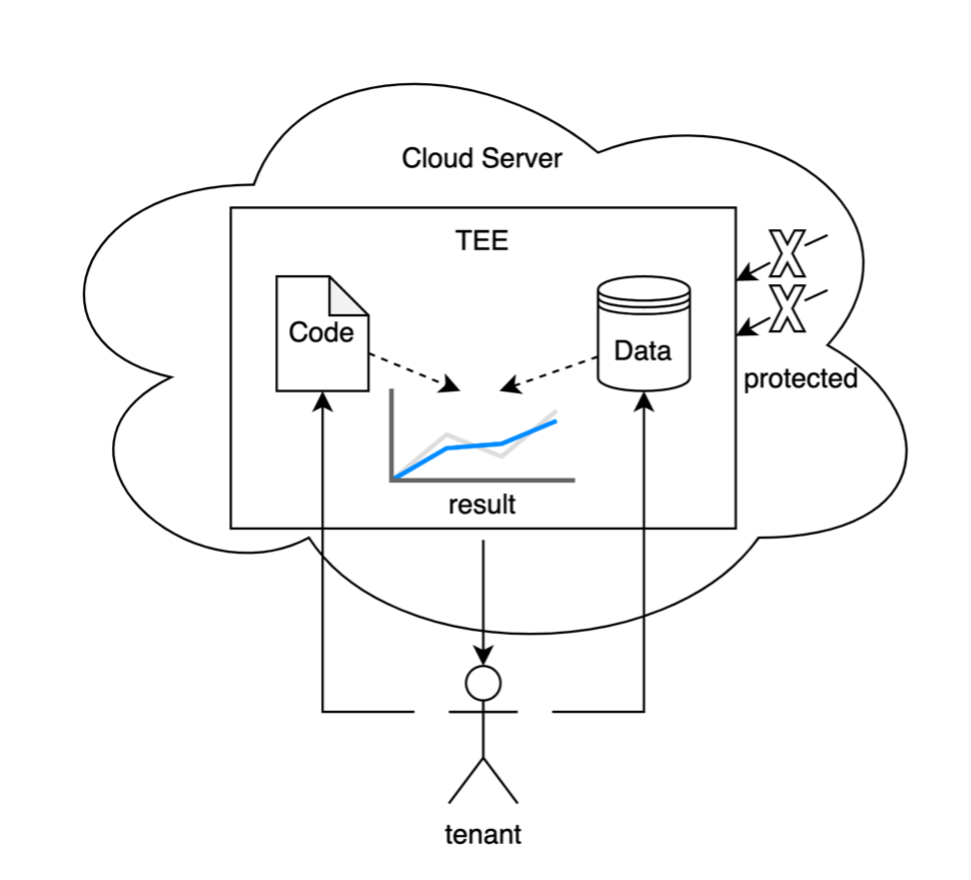
\includegraphics{images/analysis_2_roles.png}
        }
      } &
      \subfloat[多角色]{
  \hspace*{-1cm}
        \scalebox{0.42}{
        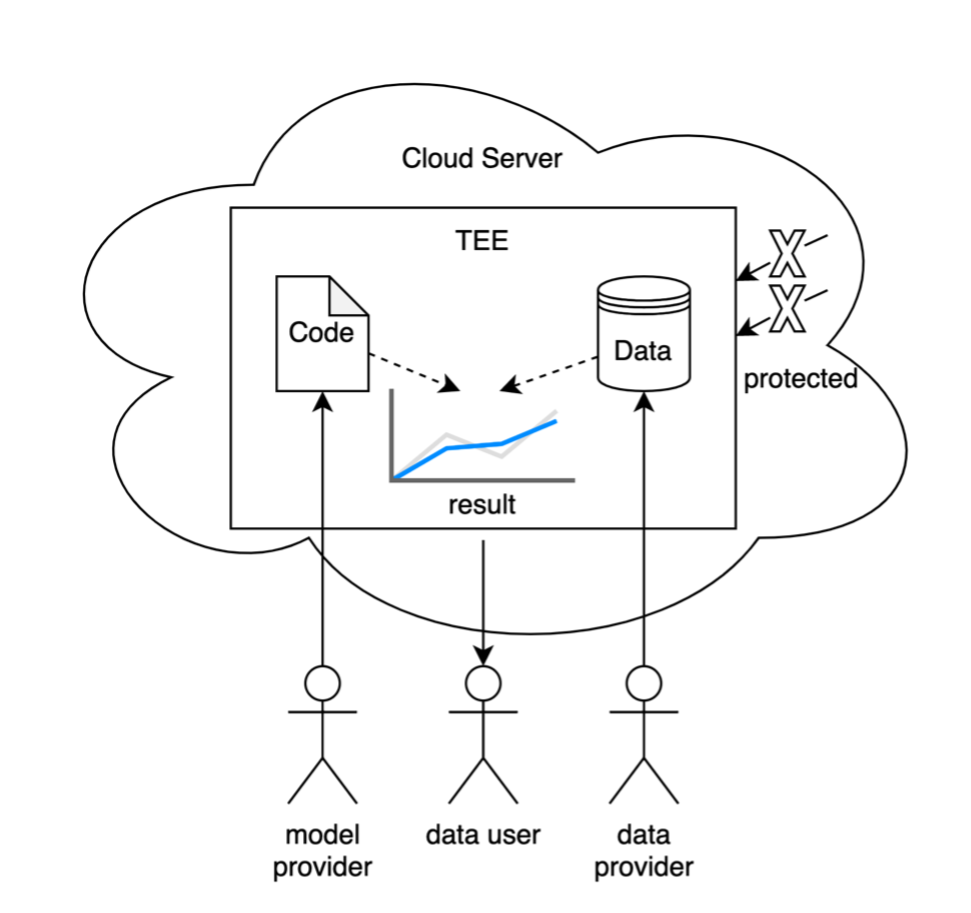
\includegraphics{images/analysis_4_roles.png}
        }
      }    \\
\end{tabular}
  }
  \caption{\small 两个角色与多角色的数据分析场景。}
  \label{fig:analysis_scenarios}
\end{figure}
% 然而,这些相关的研究在解决复杂的数据分析场景时,仍存在一些限制。
然而,这些相关研究在解决这些数据分析场景时仍存在某些限制。
% 首先,这些相关的研究工作不能保证数据分析结果中不会泄漏数据。虽然这些工作引入了数据使用规则,用以描述哪些人以什么样的价格访问哪些类型的数据,但对数据进行分析的程序是存在作恶的可能的,分析程序的最终输出结果可能是包含敏感信息泄漏的。一个最简单的例子是,分析程序直接输出原始数据,这样数据分析结果就获取到了完整的原始数据。
首先,这些相关研究工作不能保证数据分析结果中不会泄露数据。虽然这些工作引入了数据使用策略来描述谁可以以什么价格访问什么类型的数据,但数据分析程序存在恶意行为的可能性。分析程序的最终输出可能包含敏感信息的泄露。一个例子是当分析程序直接输出原始数据时,允许数据分析结果获得完整的原始数据。
% 一个straghtforward的解决方案是,要求分析程序公开,数据提供方可以审核分析程序是否存在泄漏数据的代码。但是对于模型提供方而言,模型也是他们重要的资产,他们不希望模型公开。另一方面,对于复杂的分析程序来说,审核分析程序存在巨大的工作量,不可能要求每一个分析任务都去进行审核,这会大大降低数据分析的效率。
一个直接的解决方案是要求分析程序公开,供数据提供方审计,确保它不包含可能导致数据泄露的代码。然而,对于模型提供方来说,他们的模型是有价值的资产,他们可能不愿意公开。另一方面,审计复杂的分析程序代表巨大的工作量,要求对每个分析任务进行审计是不可行的,因为这会显著降低数据分析的效率。

% 结果可验证
% 其次,当前的工作中并不能保证计算结果的可信与可验证。具体来说,数据使用方得到计算结果后,他不能确定这个计算结果确实是通过指定的数据与指定的模型运行之后得到的计算结果,而不是一个随机生成的结果。更进一步,数据使用方并没有任何方式去验证这个结果的正确性。如果计算结果的可信和可验证都无法保证,那么完全可以用一个伪造的计算结果来欺骗数据使用方,数据使用方的利益将会受到损害。
其次,现有工作无法确保计算结果的可靠性和可验证性。具体来说,当数据使用方收到计算结果时,他们无法确认这些结果确实来自通过指定模型运行指定数据,而不是简单随机生成的。此外,数据使用方缺乏任何验证这些结果正确性的方法。如果没有对计算结果的可靠性和可验证性的保证,就有可能使用欺骗性结果来误导数据使用方,损害他们的利益。

% 分析程序一致性
% 最后,当前的工作中每一次进行数据分析任务都需要使用remote attestation来保证分析程序的一致性,但是有相关工作表明,remote attestation具有低效、依赖可信第三方的缺点。
最后,在现有工作中,每个数据分析任务都需要使用远程认证来确保分析程序的一致性。然而,相关工作~\cite{chen2019opera,chen2022mage}表明,远程认证具有低效和依赖可信第三方的缺点。
% 以Intel SGX中的Enhanced Privacy ID(EPID)为例,一次remote attestation的过程会涉及到Intel Provisioning Service(IPS)、Intel Attestation(IAS) Service、Intel-signed provisioning enclave(PvE)、Intel-signed quoting enclave(QE)以及分析程序Enclave之间的交互。这些服务和Enclaves之间的交互需要通过广域网传输数据,同时,传输的数据需要加密保证其安全性,对于频繁的数据分析任务而言,性能上会有较大的损失。另一方面,IPS和IAS是Intel提供的中心化服务,remote attestation需要依赖其稳定运行。
以Intel软件保护扩展(SGX)增强隐私ID(EPID)为例,单次远程认证过程涉及Intel配置服务(IPS)、Intel认证服务(IAS)、Intel签名的配置enclave(PvE)、Intel签名的引用enclave(QE)和分析程序enclave之间的交互。这些交互需要通过广域网传输数据,传输的数据必须加密以确保其安全性。对于频繁的数据分析任务,这可能导致显著的性能开销。另一方面,IPS和IAS是Intel提供的集中式服务,使远程认证依赖于它们的稳定运行。

在本文中,我们提出了Fidelius,一个利用Intel SGX和区块链来增强数据分析安全性的系统,解决了前面提到的局限性。
% 其中,Intel SGX保证数据分析过程的security和integrity,区块链用于可信的传输、存储和验证。
Intel SGX确保数据分析过程的安全性和完整性,而区块链用于可信的传输、存储和验证。

% 为了解决计算结果泄漏数据的问题,Fidelius使用了静态二进制分析的方法,检查模型提供方的分析程序是否遵循隐私描述语言。其中,我们引入的隐私描述语言将数据的运算规则描述为有限状态机,反映了从输入数据到输出数据的状态转换,不在隐私描述语言描述的状态转换,都会被认为违反了隐私规则。
为了解决计算结果中数据泄露的问题,Fidelius采用静态二进制分析方法~\cite{schulte2019gtirb}来检查模型提供的分析程序是否遵循隐私描述语言(PDL)。在这种情况下,引入的PDL将数据的计算规则描述为有限状态机(FSM),捕获从输入数据到输出数据的状态转换。任何未在PDL中描述的状态转换都被视为违反隐私规则。

% 为了解决计算结果的可信与可验证的问题,Fidelius提供了一套密码协议,该协议中由数据使用方提供一个私钥,该私钥通过加密转发至分析程序的Enclave中,并签名计算结果。由于该私钥仅在指定的分析程序Enclave中解密获得,数据提供方、模型提供方、云计算服务提供商均无法获取,故只要被签名的计算结果能够通过验证,说明计算结果确实出自指定的分析程序且可验证。
为了确保计算结果的可靠性和可验证性,Fidelius提供了一个密码协议。在这个协议中,数据使用方提供一个私钥,该私钥安全地传输到分析程序的Enclave中并用于签名计算结果。由于这个私钥只能在指定的分析程序Enclave内解密,数据提供方、模型提供方和云服务提供商都无法访问。因此,如果签名的计算结果能够成功验证,就确认结果确实来自指定的分析程序并且是可验证的。

% 为了解决remote attestation低效、持续依赖中心化服务的问题,Fidelius结合设计的密码协议以及local attestation实现分析程序的一致性验证。Fidelius设计了密钥管理的Enclave,在初始化的过程中获取密钥的授权,在此后的所有数据分析任务中,使用该经授权的密钥执行local attestation完成分析程序的一致性验证。
为了解决远程认证的低效和持续依赖集中式服务的问题,Fidelius结合设计的密码协议和本地认证来实现分析程序的一致性验证。Fidelius引入了密钥管理Enclave,在初始化过程中获得授权密钥。随后,在所有数据分析任务中,使用这个授权密钥执行本地认证,确保分析程序的一致性。

本文的主要贡献总结如下:
\begin{itemize}
    \item \textbf{形式化安全验证机制}:我们设计了一种隐私描述语言(PDL)结合静态二进制分析,通过形式化验证确保程序行为符合预定义的安全策略,严格强制执行数据机密性,有效防止计算结果中的敏感数据泄露。
    \item \textbf{基于数字签名的密码协议}:我们提出了一种创新的密码协议,通过数字签名技术确保计算结果的可靠性、可验证性和不可否认性,解决了多角色场景中的信任问题。
    \item \textbf{高效认证机制}:我们设计了一次性远程认证与本地认证相结合的机制,显著降低了系统开销,提高了分析程序一致性验证的效率,相比传统方法减少了90\%的认证开销。
    \item \textbf{系统性能评估}:我们通过全面的实验评估证明了Fidelius的实用性,实验结果表明它产生的开销不到2\%,同时超越现有解决方案30倍以上,为实际部署提供了有力支撑。
\end{itemize} 
\section{背景}
\subsection{Intel SGX}
Intel软件保护扩展(SGX)是一个硬件级别的可信执行环境,用于保护程序执行。它建立了一个安全的私有内存区域,称为Enclave页面缓存(EPC),保护其内容免受外部进程的未授权访问或修改。这个指定的内存空间被认为是可信的,而超出它的任何区域都被视为不可信的,严格限制从不可信环境的访问。

部署在EPC内的程序被称为enclave程序。Enclaves被设计为与不可信环境隔离运行,只能通过明确声明的方法进行交互,这些方法被称为ECALL或OCALL方法。

我们将介绍封装在enclave内的关键方法和操作。
\begin{itemize}
\item $sgx\_get\_key()$: 此函数检索基于当前enclave哈希值、CPU ID和其他配置文件生成的对称密钥。每个enclave都有一个以这种方式生成的唯一对称密钥。除非声明特定的导出(OCALL)方法,否则对称密钥在enclave外部无法访问。
\item $sgx\_ecc256\_create\_key\_pair()$: 此函数通过利用SGX的自包含随机数生成器生成ECC-256非对称密钥对。
\end{itemize}

为了安全地将私有消息从enclave存储到本地存储中,"seal"操作使用enclave的对称密钥加密消息,然后本地存储。这种方法确保密封消息的明文对用户不可访问,因为对称密钥保持未公开。
为了解封消息,用户使用指定的(ECALL)方法将消息传输到enclave,enclave使用自己的对称密钥解密消息。

\subsection{远程认证}
远程认证是Intel SGX提供的一种技术,用于证明在未知平台上运行的enclave程序的完整性。目前,Intel SGX提供两种类型的远程认证:Intel增强隐私ID(Intel EPID)认证和椭圆曲线数字签名算法(ECDSA)认证。

基于EPID的远程认证通常包括以下步骤。应用程序enclave向Intel SGX提供的本地引用enclave(QE)发起请求,生成应用程序enclave的引用。这两个enclave使用本地认证进行请求发起和引用传输,其中本地认证建立可信通道并实现同一平台上两个enclave之间的数据传输。接收到引用后,应用程序enclave将其发送到远程Intel认证服务(IAS)进行验证并获得验证结果。

EPID存在一些限制,例如要求应用程序enclave所在的网络能够连接到Intel认证服务。它还要求Intel认证服务在任何时候都高可用,即不存在单点故障或停机。

基于ECDSA的认证被引入以解决与EPID相关的限制。通过Intel SGX数据中心认证原语(DCAP),基于ECDSA的认证使提供商能够建立并提供第三方认证服务,消除对Intel提供的远程认证服务的依赖。

Intel SGX DCAP允许第三方提供引用enclave并为应用程序enclave生成引用。第三方引用enclave使用的认证密钥可以在数据中心内部生成。认证密钥的公钥被发送到Intel的配置认证Enclave(PCE)并被签名/授权。生成引用后,它被发送到数据中心的内部认证服务进行验证。

SGX提供两种类型的enclave间通信:本地认证(LA)和远程认证(RA)。本地认证仅限于同一平台上的两个enclave,而远程认证促进跨平台通信。在本地认证期间,每个enclave可以验证交互enclave的哈希值或签名者。相比之下,远程认证需要可信的第三方,如Intel服务器或DCAP,来验证此信息。

\subsection{区块链}
\subsubsection{无许可链和有许可链}
区块链可以分为无许可链和有许可链。在无许可链中,所有人都可以访问,节点可以自由加入或离开,没有任何权限控制。由于无许可链的限制较少,在所有节点之间达成共识可能相对困难,导致系统吞吐量较低。无许可链最初用于跨境支付,后来发展成为去中心化金融的基础技术框架。

有许可链由多个成员组成,通常包括企业、机构、政府实体等类似组织。有许可链作为可信第三方,具有开放性和透明性的特点。它们主要用于公开数据公证、溯源、验证等。由于有许可链中的成员数量较少,可以采用高效的共识算法来促进它们之间的共识,从而使有许可链具有更高的吞吐性能。

在Fidelius中,有许可区块链的利用作为可靠且容错的第三方实体,用于数据传输、数据存储等任务。相比之下,传统中介容易受到单点故障、数据篡改风险以及建立P2P私有网络的高成本影响。

\subsubsection{智能合约}
区块链的智能合约是链上程序,以其代码和执行过程的透明度而闻名。在Fidelius中,智能合约在验证云服务提供商提供的分析结果签名方面发挥着关键作用。一旦验证成功完成,数据分析的成功就得到保证,为所有相关方建立信任。 
\section{威胁模型与设计选择}

在本节中,我们首先介绍系统中的角色,然后详细说明威胁模型,突出潜在风险并讨论各种类型的攻击。此外,我们建立关键假设,这些假设构成了Fidelius设计和实施的基础。随后,我们深入探讨为Fidelius做出的设计选择,旨在缓解已识别的风险并应对系统上的潜在攻击。

\subsection{角色}
\begin{itemize}
    \item 数据提供方(DP)。数据提供方作为原始数据的唯一所有者,最初在区块链上发布元数据,包括哈希值和原始数据的必要描述。此元数据的准确性通过数据提供方的可信度进行验证,以成功数据分析的历史为例。
    \item 模型提供方(MP)。模型提供方为特定类型的数据提供分析程序。
    \item 云服务提供方(CSP)。云计算提供方提供数据分析所需的计算资源,并额外提供可信执行环境以确保安全的数据分析。在接收到数据分析任务请求后,云计算提供方有义务执行分析程序并将结果返回给区块链。
    \item 数据使用方(DU)。数据使用方通过检查区块链上的元数据选择所需的原始数据,并启动数据分析以从指定的分析程序获得结果。
    \item 区块链。区块链作为数据传输和存储的可靠、抗故障的第三方。具体而言,智能合约验证分析结果上签名的正确性。
\end{itemize}

\subsection{威胁模型}
系统包含数据提供方、模型提供方、云服务提供方以及数据使用方四个角色,四个角色之间是相互不信任的。

在数据分析的过程中,存在以下攻击:
\begin{itemize}
    \item 数据窃取攻击:云服务提供方可能通过他们提供的硬件或软件资源窃取数据;数据使用方可能登录服务器窃取数据。模型提供方提供的程序可能包含旨在窃取原始或中间数据的恶意代码。
    \item 数据伪造攻击:数据提供方提供的数据与声称的不一致。
    \item 数据滥用攻击:数据提供方的数据在没有适当授权的情况下被用于不同的模型和云服务器。
    \item 结果伪造攻击:数据分析的结果并不准确反映模型的真实执行。
    \item 结果窃取攻击:数据分析的结果被数据提供方、模型提供方、云服务提供方或未知的攻击者非法获取。
\end{itemize}

我们在本文中不解决Intel SGX的侧信道攻击。我们假设Intel SGX的硬件功能如广告所示,确保enclave内的代码保持不变,内部变量的值受到保护,免受直接内存访问。值得注意的是,我们对Intel的依赖仅限于设置过程中的一次性交互;不需要与Intel服务器或DCAP进行进一步联系。相比之下,以前的方法依赖远程认证,要求Intel服务器或DCAP在每个数据分析任务中持续保持完整性和可用性。

我们假设存在抗碰撞哈希函数和安全签名及加密方案。具体而言,我们的签名包含\textit{nonce},确保有效的签名对$(msg, signed_{msg})$不能由没有私钥的对手生成,使历史签名无效。

\subsection{设计选择}
为了应对已识别的攻击,我们做出了以下设计选择。
\begin{itemize}
    \item 抵御数据窃取攻击:所有存在于非可信环境(例如网络传输、云服务器的非TEE部分)的数据都经过加密处理,以防止数据使用方或云服务提供商直接窃取数据。模型提供方提供的分析程序,在进行数据分析前进行代码静态分析,防止模型提供方通过数据分析结果窃取数据。
    \item 抵御数据伪造攻击:执行数据分析前,检查数据哈希与声称的哈希是否一致。
    \item 抵御数据滥用攻击:引入数字签名技术,数据提供方用私钥签名使用数据的平台、模型以及模型的参数,在执行数据分析前,会验证该签名的有效性。
    \item 抵御结果伪造攻击:将数据使用方的私钥加密地传输到云服务器的可信执行环境中,并用这个私钥签名结果。当数据使用方拿到结果时,也会得到该私钥对结果的签名,若签名验证通过,说明结果确实是由可信执行环境中得到的,故结果未经伪造。这一思想类似于零知识证明。
    \item 抵御结果窃取攻击:数据分析结果由数据使用方的公钥加密,只能被数据使用方查看。
\end{itemize} 
\section{设计}

\subsection{概述}
本节简要概述Fidelius中使用的enclaves和符号,以及其架构和工作流程。

\subsubsection{Enclaves和符号}
在本文中,我们定义以下enclaves和符号:
\begin{itemize}
    \item EKeyMgr。Enclave密钥管理器管理非对称密钥,处理创建、删除并提供基本密码学功能,包括消息加密、解密、签名和签名验证。
    \item EAnalyzer。Enclave分析器,一个Intel SGX Enclave格式的分析程序,确保程序在执行期间保持不变。
    \item $(PK_{DP},SK_{DP})$,数据提供方的非对称密钥对。
    \item $(PK_{DU},SK_{DU})$,数据使用方的非对称密钥对。
    \item $(PK_{CSP}, SK_{CSP})$表示云服务提供方的非对称密钥对,由EKeyMgr生成。私钥$SK_{CSP}$安全地存储在enclave内,确保云服务提供商无法提取。
    \item $H(\cdot)$表示哈希函数。
    \item $Enc(PK, msg)$表示使用$PK$加密$msg$。
    \item $Dec(SK, cipher)$表示使用$SK$解密$cipher$。
    \item $Sign(SK, msg)$表示使用$SK$对$msg$进行签名。
    \item $Verf(PK, msg, sig)$表示使用$PK$和$msg$验证$sig$。
    \item $\mathcal{F}(SK, PK_{CSP}, H_{EA})$表示使用$PK_{CSP}$将$SK$转发到EKeyMgr的过程。在此上下文中,$SK$在EAnalyzer中使用,由$H_{EA}$标识。函数$\mathcal{F}(\cdot)$涉及$Sign(SK, concat(PK_{CSP}, H_{EA}))$和$Enc(PK_{CSP}, SK)$。
\end{itemize}

\subsubsection{架构和工作流程}

Fidelius架构和数据分析工作流程如图所示。
该过程从设置阶段开始,其中CSP中的EKeyMgr生成非对称密钥对。公钥$PK_{CSP}$通过Intel的远程认证服务进行验证,而私钥$SK_{CSP}$安全地存储在EKeyMgr内。同时,数据提供方(DP)和数据使用方(DU)各自生成自己的非对称密钥对,并保留这些密钥。此外,DP使用她的公钥$PK_{DP}$加密数据,并为DU的使用准备这些加密数据。

DP将加密数据上传到CSP,并使用$\mathcal{F}(SK_{DP}, PK_{CSP}, H_{EA})$将她的私钥$SK_{DP}$转发给EKeyMgr。类似地,DU将分析程序上传到CSP,并使用相同的方法将她的私钥$SK_{DU}$转发给EKeyMgr。重要的是要注意,明文私钥($SK_{DP}$和$SK_{DU}$)只能在EKeyMgr内解密。

一旦分析程序、加密数据和私钥准备就绪,数据分析任务就开始了。首先根据隐私描述语言(PDL)定义的规则检查分析程序。任何未通过此检查的程序都会导致分析任务立即终止。随后,EAnalyzer加载并解密加密数据。然后验证解密数据的哈希值;如果与声称的哈希不匹配,EAnalyzer立即停止以防止处理被篡改或欺诈的数据。如果数据得到验证,EAnalyzer继续进行主要分析,最终使用$PK_{DU}$产生加密结果。此外,使用$SK_{DU}$对结果进行签名。由于$SK_{DU}$位于EKeyMgr内,EAnalyzer通过本地认证建立安全通道来请求$SK_{DU}$。

\subsection{隐私描述语言}
为了防止数据分析结果泄漏数据,我们提出了隐私描述语言来定义使用数据的规则,并通过了静态二进制分析的方法检查分析程序是否遵守隐私描述语言定义的规则。如图所示,这段代码使用PDL描述了在Iris数据集上使用Kmeans算法的规则,这段代码也将被转换成LLVM的中间表示,然后使用符号执行得到PDL描述的规则的状态a。另一方面,我们使用GTIRB作为分析的中间表示,在将分析程序转换为中间表示后,使用符号执行获取每个输出变量的状态b,并判断是否满足b包含于a。

\subsection{可信和可验证的结果}
算法概述了EKeyMgr和EAnalyzer的主要操作。在EAnalyzer内生成的加密分析结果及其签名被传输到区块链。在那里,任何人都可以验证签名的有效性。有效的签名确认DP成功执行了分析程序并获得了正确的结果,因为签名源自EAnalyzer内部。这种机制防止攻击者在未执行分析程序的情况下伪造有效签名,从而确保数据分析过程的完整性。DU可以从区块链下载加密结果,并使用$SK_{DU}$解密以获得明文分析结果。

\subsection{一次性远程认证}
我们实施一次性远程认证过程,从一开始就建立安全和可信的环境。在设置阶段,云服务提供商(CSP)通过与Intel认证服务进行远程认证来验证EKeyMgr生成的公钥$PK_{CSP}$的授权。这种彻底的验证确认了CSP凭据的完整性和合法性。一旦验证完成,CSP上的后续分析任务不再需要远程认证。DP和DU转发的私钥($SK$)通过本地认证从EKeyMgr安全传输到EAnalyzer。 
\section{评估}\label{sec:eval}
\SetKwInput{KwForEach}{for each}
\begin{algorithm}[h]
    \caption{一次性远程认证}
    \KwIn{NULL}
    $(PK_{CSP}, SK_{CSP}) \gets sgx\_ecc256\_create\_key\_pair()$\;
    向Intel服务进行远程认证以验证$PK_{CSP}$的授权\;
    \KwForEach{数据分析任务}
    \Begin{
        $SK \gets Dec(SK_{CSP},Enc_{SK})$\;
        在EKeyMgr和EAnalyzer之间建立本地认证通道\;
        使用$SK$\;
    }
    \KwRet{}\;
\label{algo:attestation}
\end{algorithm} 

在本节中,我们通过综合实验评估Fidelius的性能。首先,我们通过分别执行CPU密集型和I/O密集型任务来评估其时间消耗。随后,我们对Fidelius与在以太坊虚拟机(EVM)中执行分析程序的替代解决方案进行性能比较。我们的实验在一台配备Intel(R) Core(TM) i5-10400F CPU的机器上进行,该CPU拥有12个核心,频率为2.9 GHz,16 GB内存和12 MB缓存。除非另有说明,每个实验重复1,000次以计算平均值。

\subsection{CPU密集型任务}
为了评估Fidelius在CPU密集型任务上的性能,我们实现了一个具有三层和128个隐藏单元的神经网络算法,设计用于使用MNIST数据集识别手写数字~\cite{mnist}。我们报告算法的时间消耗和准确性。此外,我们在原始CPU(无SGX)上部署算法进行比较。基于Fidelius的算法与基于原始CPU的算法之间的主要差异包括:
\begin{itemize}
  \item 随机库。基于Fidelius的算法使用基于Intel SGX的随机库,而基于原始CPU的算法依赖C++随机库。
  \item 数据解密。Fidelius在启动算法前需要解密密封数据,产生额外的处理时间。相反,基于原始CPU的算法可以直接访问明文数据。
\end{itemize}
对于Fidelius和原始CPU,我们保持固定的测试集数量为1,000,同时将训练集数量从10,000逐步增加到50,000。对于每个训练集,我们分别将epoch设置为100和200来执行算法。

\begin{figure*}[h]
\centering
{
  \setlength{\tabcolsep}{0pt}
  \begin{tabular}{cccc}
\subfloat[epoch = 100]{
  \scalebox{0.39}{
  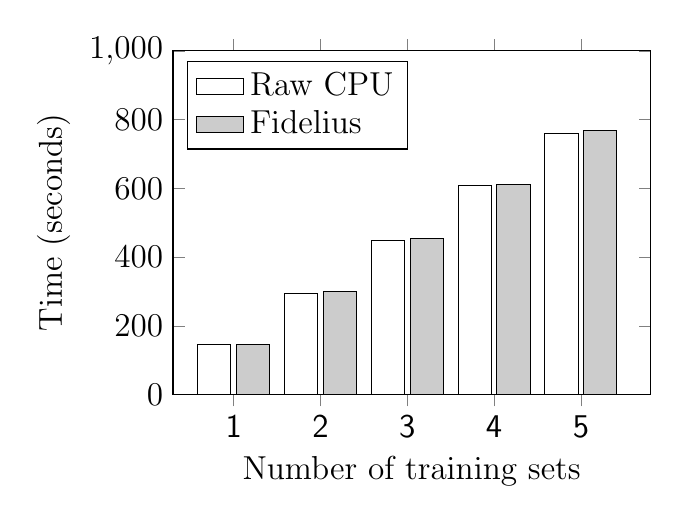
\begin{tikzpicture}
    
\begin{axis}[
  compat=newest,
  legend style={
     legend columns=1,
     font=\large,
     legend pos=north west},
  ybar,
  bar width=12pt,
  ymin=0,
  ymax=1000,
  xmin=0.3,
  xmax=5.8,
  scale only axis,
  xticklabels={\bench{\large 1}, \bench{\large 2}, \bench{\large 3},
    \bench{\large 4}, \bench{\large 5}
  },
  ylabel={Time (seconds)
  },
    xlabel=Number of training sets,
    xtick=data,
    width=0.5\textwidth,
    height=0.36\textwidth,
    every axis/.append style={font=\large,
      label style={font=\large},
      tick label style={font=\large}
    }
  ]
\addplot [area legend] coordinates{
  (1, 144.6828)
  (2, 293.267)
  (3, 447.979)
  (4, 609.104)
  (5, 758.237)
};
\addplot [fill=black!20,area legend] coordinates{
  (1, 145.0)
  (2, 298.95)
  (3, 454.3)
  (4, 612.15)
  (5, 768.33)
};
\legend{[right]{Raw CPU}, [right]{Fidelius}}
\end{axis}
\end{tikzpicture}}
} &
\subfloat[epoch = 200]{
  \scalebox{0.39}{
  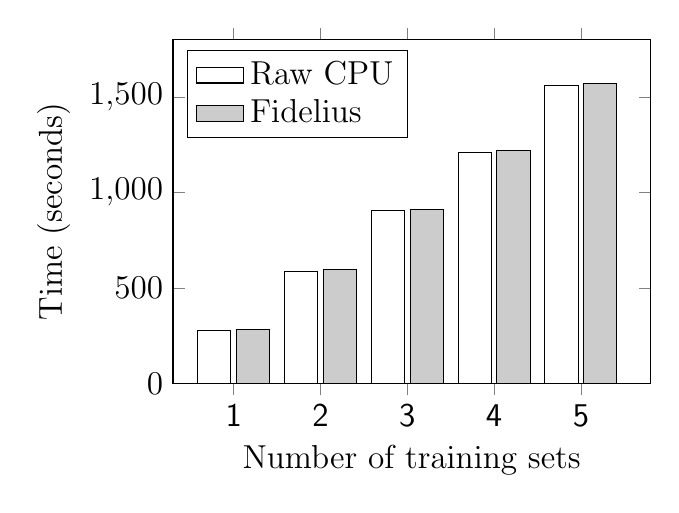
\begin{tikzpicture}
    
\begin{axis}[
  compat=newest,
  legend style={
     legend columns=1,
     font=\large,
     legend pos=north west},
  ybar,
  bar width=12pt,
  ymin=0,
  ymax=1800,
  xmin=0.3,
  xmax=5.8,
  scale only axis,
  xticklabels={\bench{\large 1}, \bench{\large 2}, \bench{\large 3},
    \bench{\large 4}, \bench{\large 5}
  },
  ylabel={Time (seconds)
  },
    xlabel=Number of training sets,
    xtick=data,
    width=0.5\textwidth,
    height=0.36\textwidth,
    every axis/.append style={font=\large,
      label style={font=\large},
      tick label style={font=\large}
    }
  ]
\addplot [area legend] coordinates{
  (1, 278.258)
  (2, 587.359)
  (3, 905.65)
  (4, 1208.9)
  (5, 1562.5)
};
\addplot [fill=black!20,area legend] coordinates{
  (1, 282)
  (2, 595.27)
  (3, 909.03)
  (4, 1219.71)
  (5, 1570)
};

\legend{[right]{Raw CPU}, [right]{Fidelius}}
\end{axis}		
\end{tikzpicture}}
} &
\subfloat[epoch = 100]{
  \scalebox{0.39}{
  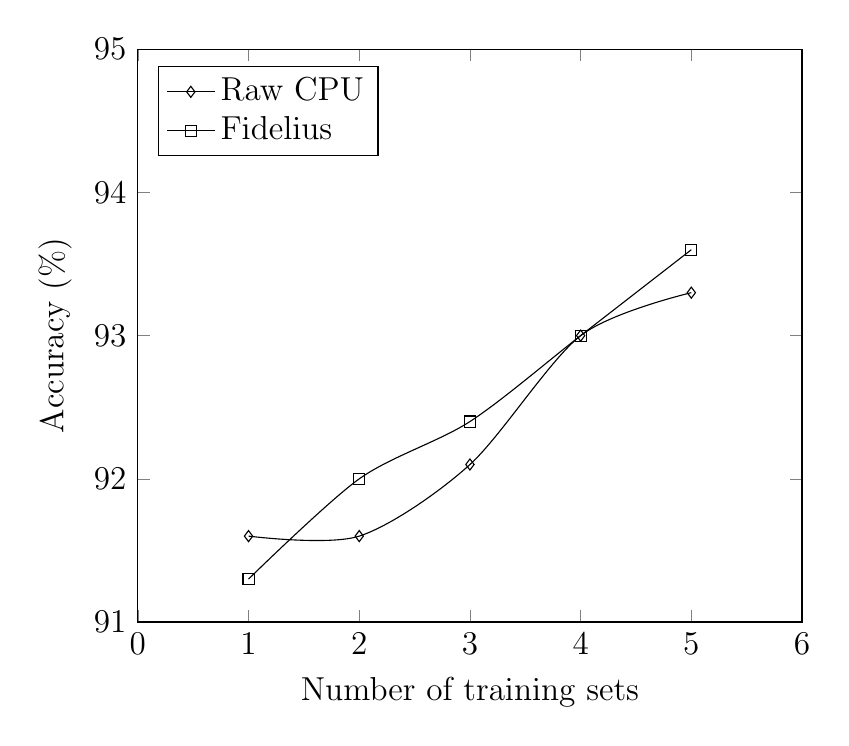
\begin{tikzpicture}
    
\large
\pgfplotsset{
    scale only axis,
    xmin=0, xmax=6,
    compat=newest,
    legend pos=north west,
}

\begin{axis}[
  %axis y line*=left,
  %scaled y ticks=base 10:2,
  %ymin=0, ymax=0.0004,
  %ymin=0, ymax=0.008,
  ymin=91, ymax=95,
  xlabel=Number of training sets,
  %width=0.4\textwidth,
  %height=0.6\textwidth,
  ylabel=Accuracy (\%),
]

\addplot[smooth,mark=diamond]
  coordinates{
    (1,91.6)
    (2,91.6)
    (3,92.1)
    (4,93.0)
    (5,93.3)
}; \label{plot_raw}

\addplot[smooth,mark=square]
  coordinates{
    (1,91.3)
    (2,92.0)
    (3,92.4)
    (4,93.0)
    (5,93.6)
  }; \label{plot_fid}



  \addlegendimage{/pgfplots/refstyle=plot_raw}\addlegendentry[right]{Raw CPU}
  \addlegendimage{/pgfplots/refstyle=plot_fid}\addlegendentry[right]{Fidelius}

\end{axis}
\end{tikzpicture}}
} &
\subfloat[epoch = 200]{
  \scalebox{0.39}{
  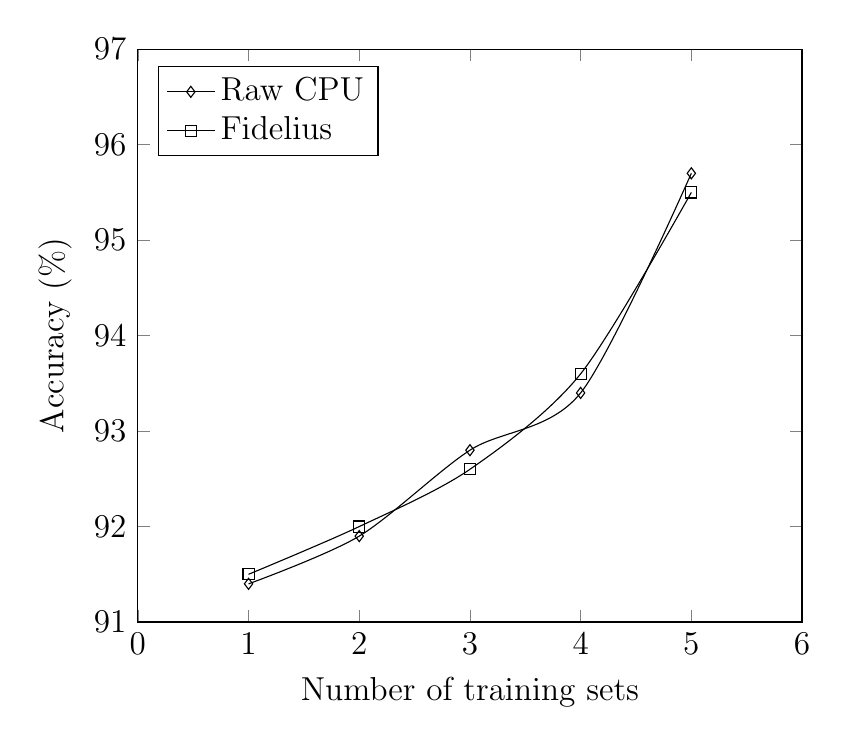
\begin{tikzpicture}
    
\large
\pgfplotsset{
    scale only axis,
    xmin=0, xmax=6,
    compat=newest,
    legend pos=north west,
}

\begin{axis}[
  %axis y line*=left,
  %scaled y ticks=base 10:2,
  %ymin=0, ymax=0.0004,
  %ymin=0, ymax=0.008,
  ymin=91, ymax=97,
  xlabel=Number of training sets,
  %width=0.4\textwidth,
  %height=0.6\textwidth,
  ylabel=Accuracy (\%),
]

\addplot[smooth,mark=diamond]
  coordinates{
    (1,91.4)
    (2,91.9)
    (3,92.8)
    (4,93.4)
    (5,95.7)
}; \label{plot_raw}

\addplot[smooth,mark=square]
  coordinates{
    (1,91.5)
    (2,92.0)
    (3,92.6)
    (4,93.6)
    (5,95.5)
  }; \label{plot_fid}



  \addlegendimage{/pgfplots/refstyle=plot_raw}\addlegendentry[right]{Raw CPU}
  \addlegendimage{/pgfplots/refstyle=plot_fid}\addlegendentry[right]{Fidelius}

\end{axis}
\end{tikzpicture}}
} \\
\end{tabular}
}
  \caption{\small CPU密集型任务的时间消耗和准确性。}
\label{fig:cpu_intensive}
\end{figure*} 

图~\ref{fig:cpu_intensive}(a)和~\ref{fig:cpu_intensive}(b)说明了在不同epoch下在Fidelius和原始CPU上运行的算法的时间消耗。随着训练集数量的增加,Fidelius和原始CPU上算法的时间消耗都呈现线性增长趋势。然而,这两种算法之间的时间消耗差异很小。具体而言,观察到Fidelius上的执行时间仅比原始CPU长2\%,主要是由于数据解密开销。

图~\ref{fig:cpu_intensive}(c)和~\ref{fig:cpu_intensive}(d)显示了在不同epoch下Fidelius和原始CPU上算法的准确性,两者都达到了超过91\%的准确性。在100个epoch时,准确性略有波动,但平台之间没有明显差异。在200个epoch时,两种算法都收敛到几乎相同的准确性。Fidelius与原始CPU相比时间消耗增加了2\%,但保持了相似的准确性水平,在CPU密集型任务中表现出可比的性能。

\subsection{I/O密集型任务}\label{subsec:io_intensive}
为了评估Fidelius在处理I/O密集型任务时的时间效率,我们在Fidelius和原始CPU平台上测试了一个在超过1 GB文件中搜索目标字符串的算法。时间消耗取决于数据加载和字符串搜索,Fidelius由于数据解密需要额外时间。考虑到Intel SGX在Fidelius中的约束,我们将数据加载块大小设置为64 KB和256 KB,并为每个块大小改变数据行数从1到128和1到256来测量时间效率。

\begin{figure}[h]
  \centering
{
\begin{tabular}{cc}
      \subfloat[数据块大小 = 64 KBytes]{
        \scalebox{0.39}{
          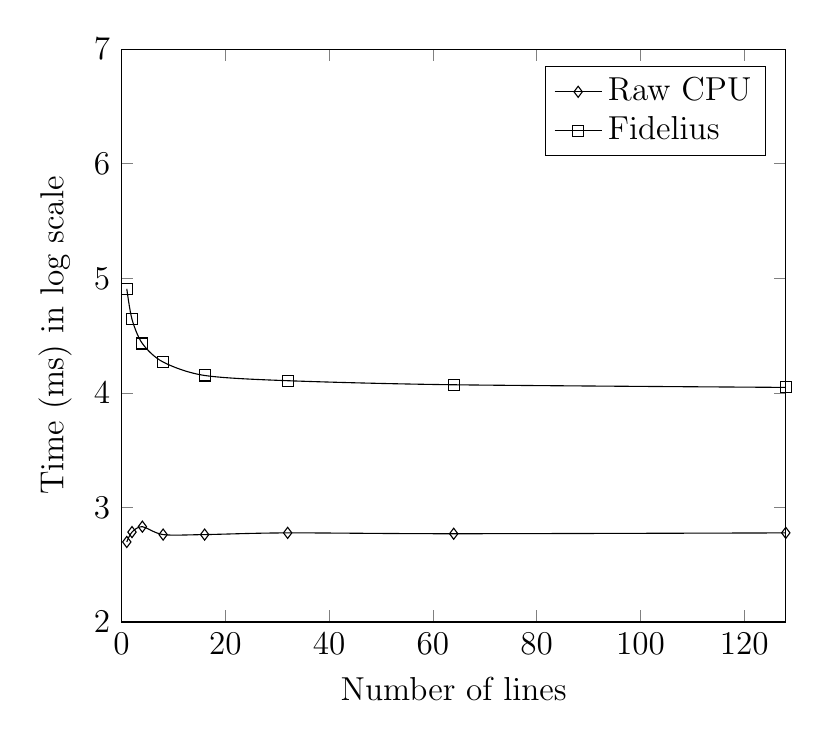
\begin{tikzpicture}
            
\large
\pgfplotsset{
    scale only axis,
    xmin=0, xmax=128,
    compat=newest,
    legend pos=north east,
}

\begin{axis}[
  %axis y line*=left,
  %scaled y ticks=base 10:2,
  %ymin=0, ymax=0.0004,
  %ymin=0, ymax=0.008,
  ymin=2, ymax=7,
  xlabel=Number of lines,
  %width=0.4\textwidth,
  %height=0.6\textwidth,
  ylabel=Time (ms) in log scale,
]

\addplot[smooth,mark=diamond]
  coordinates{
    (1,2.6990) %log10(500)
    (2,2.7853) %log10(610)
    (4,2.8325) %log10(680)
    (8,2.7634) %log10(580)
    (16,2.7634) %log10(580)
    (32,2.7782) %log10(600)
    (64,2.7709) %log10(590)
    (128,2.7782) %log10(600)
}; \label{plot_raw}

\addplot[smooth,mark=square]
  coordinates{
    (1,4.9085) %log10(81000)
    (2,4.6435) %log10(44000)
    (4,4.4314) %log10(27000)
    (8,4.2695) %log10(18600)
    (16,4.1523) %log10(14200)
    (32,4.1065) %log10(12780)
    (64,4.0711) %log10(11780)
    (128,4.0481) %log10(11170)
  }; \label{plot_fid}



  \addlegendimage{/pgfplots/refstyle=plot_raw}\addlegendentry[right]{Raw CPU}
  \addlegendimage{/pgfplots/refstyle=plot_fid}\addlegendentry[right]{Fidelius}

\end{axis}
          \end{tikzpicture}
        }
      } &
      \subfloat[数据块大小 = 256 KBytes]{
        \scalebox{0.39}{
          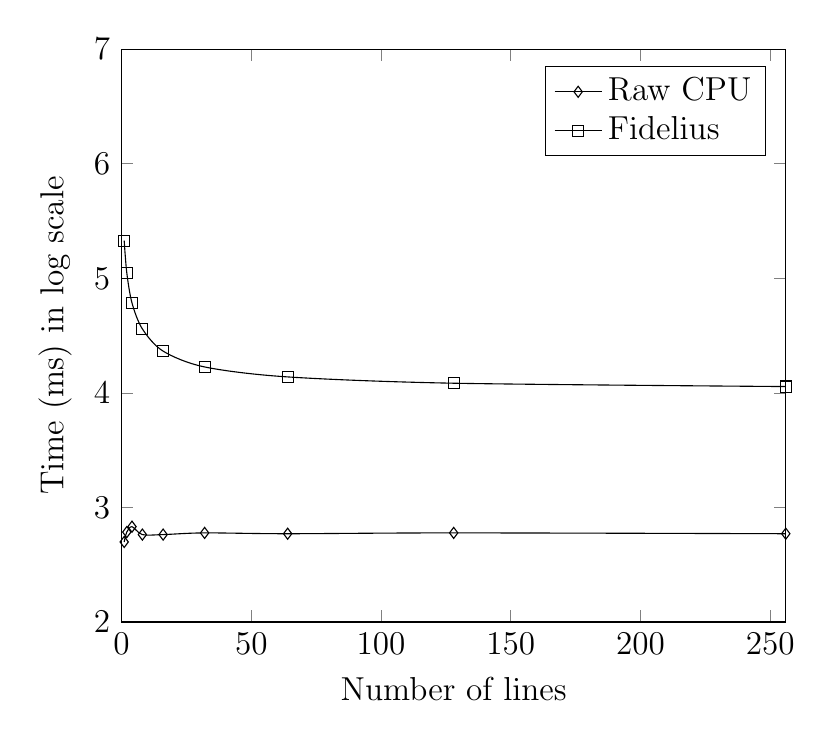
\begin{tikzpicture}
            
\large
\pgfplotsset{
    scale only axis,
    xmin=0, xmax=256,
    compat=newest,
    legend pos=north east,
}

\begin{axis}[
  %axis y line*=left,
  %scaled y ticks=base 10:2,
  %ymin=0, ymax=0.0004,
  %ymin=0, ymax=0.008,
  ymin=2, ymax=7,
  xlabel=Number of lines,
  %width=0.4\textwidth,
  %height=0.6\textwidth,
  ylabel=Time (ms) in log scale,
]
1	0.5	    213
2	0.61	111.78
4	0.68	61.04
8	0.58	36.2
16	0.58	23.16
32	0.6	    16.85
64	0.59	13.79
128	0.6	    12.15
256	0.59	11.36
\addplot[smooth,mark=diamond]
  coordinates{
    (1,2.6990) %log10(500)
    (2,2.7853) %log10(610)
    (4,2.8325) %log10(680)
    (8,2.7634) %log10(580)
    (16,2.7634) %log10(580)
    (32,2.7782) %log10(600)
    (64,2.7709) %log10(590)
    (128,2.7782) %log10(600)
    (256, 2.7709) %log10(590)
}; \label{plot_raw}

\addplot[smooth,mark=square]
  coordinates{
    (1,5.3284) %log10(213000)
    (2,5.0484) %log10(111780)
    (4,4.7856) %log10(61040)
    (8,4.5587) %log10(36200)
    (16,4.3647) %log10(23160)
    (32,4.2266) %log10(16850)
    (64,4.1396) %log10(13790)
    (128,4.0846) %log10(12150)
    (256,4.0554) %log10(11360)
  }; \label{plot_fid}



  \addlegendimage{/pgfplots/refstyle=plot_raw}\addlegendentry[right]{Raw CPU}
  \addlegendimage{/pgfplots/refstyle=plot_fid}\addlegendentry[right]{Fidelius}

\end{axis}
          \end{tikzpicture}
        }
      }    \\
\end{tabular}
  }
  \caption{\small I/O密集型任务的时间消耗。}
  \label{fig:io_intensive}
\end{figure} 
图~\ref{fig:io_intensive}显示了Fidelius与原始CPU在不同数据块大小下的时间效率比较。随着读取行数的增加,Fidelius的时间消耗显著减少。例如,在64 KB块大小时,Fidelius的时间从81秒(1行)下降到11秒(128行)。类似地,在256 KB块大小时,从213秒(1行)减少到10秒(256行)。将块大小增加到256 KB进一步优化了Fidelius的性能。尽管有所改进,Fidelius与原始CPU之间的时间消耗仍存在差距,主要是由于I/O密集型任务中的解密过程。

\subsection{性能比较}\label{subsec:evm_cmp}
在本节中,我们将Fidelius与SDTE~\cite{dai2019sdte}的性能进行比较,SDTE使用\textit{k}-最近邻(\textit{k}-NN)算法作为以太坊智能合约在以太坊虚拟机(EVM)上执行机器学习任务。我们在Fidelius和原始CPU上实现\textit{k}-NN算法来评估每个解决方案的时间消耗,使用来自Kaggle的Titanic数据集作为输入。

为了评估\textit{k}-NN算法在以太坊虚拟机(EVM)上的执行时间,我们在Ganache(个人以太坊区块链)上部署了\textit{k}-NN智能合约。报告的EVM上\textit{k}-NN的时间消耗仅关注执行时间,不包括交易广播或提交所花费的时间。我们还排除了将Titanic数据集上传到区块链所需的时间,因为\textit{k}-NN合约使用链上数据。由于EVM的内存限制,\textit{k}-NN算法无法处理超过60个测试集,因此我们将测试集限制在10-60个,同时保持训练集为100个。

\begin{figure}[h]
\centering
\scalebox{.8}
{
\begin{tikzpicture}
    
\pgfplotsset{
    scale only axis,
    xmin=0, xmax=70,
    ymin=1, ymax=5,
    compat=newest,
    legend pos=north west,
}

\begin{axis}[
  %axis y line*=left,
  %scaled y ticks=base 10:2,
  x=0.1cm,
  y=1cm,
  xlabel=测试集数量,
  %width=0.4\textwidth,
  %height=0.6\textwidth,
  ylabel=时间 (ms) 对数刻度,
]

\addplot[smooth,mark=diamond]
  coordinates{
    (10,1.1501) %log10(14.13)
    (20,1.3642) %log10(23.13)
    (30,1.5083) %log10(32.23)
    (40,1.6076) %log10(40.51)
    (50,1.6771) %log10(47.54)
    (60,1.7350) %log10(54.32)
}; \label{plot_raw}

\addplot[smooth,mark=square]
  coordinates{
    (10,1.2276) %log10(16.89)
    (20,1.4096) %log10(25.68)
    (30,1.5535) %log10(35.77)
    (40,1.6350) %log10(43.15)
    (50,1.7088) %log10(51.14)
    (60,1.7693) %log10(58.79)
  }; \label{plot_fid}

\addplot[smooth,mark=triangle]
  coordinates{
    (10,2.7589) %log10(574)
    (20,2.9425) %log10(876)
    (30,3.0449) %log10(1109)
    (40,3.1261) %log10(1337)
    (50,3.1976) %log10(1576)
    (60,3.2813) %log10(1911)
  }; \label{plot_evm}


  \addlegendimage{/pgfplots/refstyle=plot_raw}\addlegendentry[right]{原始CPU}
  \addlegendimage{/pgfplots/refstyle=plot_fid}\addlegendentry[right]{Fidelius}
  \addlegendimage{/pgfplots/refstyle=plot_evm}\addlegendentry[right]{EVM}

\end{axis}
\end{tikzpicture}
}
  

  \caption{\small 原始CPU、Fidelius和EVM上的时间消耗。}
\label{fig:knn_cmp}
\end{figure} 
图~\ref{fig:knn_cmp}显示了\textit{k}-NN算法在原始CPU、Fidelius和以太坊虚拟机(EVM)上的时间消耗,后者比其他的大约长30倍。此外,由于内存约束,EVM执行在测试超过60个集时经常失败,突出了在EVM上运行具有大数据集的复杂机器学习算法的困难,正如之前关于以太坊内存限制的研究所指出的那样~\cite{dinh2017blockbench}。相比之下,Fidelius为复杂的机器学习任务提供了更可靠和稳定的环境。 
\section{相关工作}\label{sec:related}
GXS~\cite{gxchain}作为一个基于区块链的数据交易平台运行,记录并促进买卖双方之间的交易,双方在相互同意后通过私有渠道交换数据。
AccountTrade~\cite{accounttrade}使用区块链将分析器与数据提供方配对,并通过可执行的协议和数据索引确保生态系统安全,这些协议和索引检测并惩罚不诚实的行为。
Zhao等人~\cite{zhao}开发了一个专注于提供方隐私的数据交易系统,采用环签名和双重认证来保护交易并防止未授权访问。

在数据共享系统中~\cite{dong2015secure,yue2017big,xia2017medshare},Shen等人~\cite{shen}开发了一个确保数据完整性和机密性的方案。
Zuo等人~\cite{FG}引入了一个系统,使用代理重加密和密钥分离高效保护和撤销卖方的密钥,通过基于属性的加密增强数据保护。
为了缓解恶意代理参与数据泄露,Guo等人~\cite{APRE}提出了可问责代理重加密(APRE),这是一个检测和解决重加密密钥滥用的框架,进一步验证了其在DBDH假设下的CPA安全性和可问责性。
Deng等人~\cite{IBET}形式化了一个基于身份的加密转换(IBET)模型,用于与数据所有者初始指定之外的额外接收者共享加密数据。

SDTE~\cite{dai2019sdte}引入了一个基于区块链的数据分析平台,数据提供方加密数据并上传到区块链。数据使用方选择这些数据,形成分析合约并请求服务。获得批准后,提供方通过Intel SGX远程认证将解密密钥发送给可信节点,然后该节点解密数据并在Intel SGX保护的以太坊虚拟机(EVM)中运行分析,然后将结果上传到结算合约。
然而,SDTE的加密数据上传对区块链施加了显著的存储需求,并且作为以太坊智能合约运行分析引入了性能挑战。在EVM上运行复杂的算法如\textit{k}-NN,如第~\ref{subsec:evm_cmp}节所示,由于数据规模和任务复杂性,通常是不实际的。

PrivacyGuard~\cite{xiao2020privacyguard}通过将链上分析转移到链外可信执行环境(TEE)来缓解以太坊虚拟机(EVM)的性能限制,允许数据提供方设置限制未授权数据使用的策略。然而,它仍然遇到EVM性能的挑战。类似地,Sterling~\cite{hynes2018demonstration}引入了一个利用机器学习进行数据分析的去中心化数据市场,但也像SDTE和PrivacyGuard一样对区块链施加了显著的存储需求。此外,隐私担忧或法规可能阻止敏感数据的上传。 
\section{结论}\label{sec:conclude}
%We introduced Fidelius, a novel system designed to enhance the security of data analysis in complex scenarios involving multiple roles. Leveraging Intel SGX and blockchain technology, Fidelius addresses the challenges of data leakage, trustworthiness, and verifiability of computation results. By employing static binary analysis and a privacy description language (PDL), Fidelius prevents data leakage in computation results, while its cryptographic protocol ensures the trustworthiness and verifiability of these results. Additionally, Fidelius utilizes local attestation to achieve consistent verification of analysis programs, reducing reliance on centralized services and improving efficiency. Experimental results demonstrate that Fidelius incurs minimal overhead while outperforming existing solutions. Overall, Fidelius presents a promising approach to enhance the security of data analysis, offering a robust solution for protecting sensitive data in diverse and complex scenarios.
我们提出了Fidelius,一个基于形式化验证和密码协议的多角色安全数据分析系统。Fidelius通过三个核心技术贡献解决了多角色数据分析场景中的安全挑战:(1)设计了结合静态二进制分析的隐私描述语言(PDL),通过形式化验证确保程序行为符合预定义的安全策略,有效防止计算结果中的数据泄露;(2)提出了基于数字签名的密码协议,确保计算结果的可靠性、可验证性和不可否认性;(3)设计了一次性远程认证与本地认证相结合的机制,相比传统方法减少了90\%的认证开销。实验结果表明,Fidelius在性能方面超越了现有解决方案30倍以上,同时产生的开销不到2\%,为实际部署提供了有力支撑。Fidelius为多角色复杂场景中的数据分析安全性提供了一个实用且高效的解决方案,具有重要的理论价值和实际应用前景。 

%%
%% The next two lines define the bibliography style to be used, and
%% the bibliography file.
\bibliographystyle{ACM-Reference-Format}
\bibliography{sample-base}


%%
%% If your work has an appendix, this is the place to put it.

\end{document}
\endinput
%%
%% End of file `sample-sigconf-chinese.tex'.